\documentclass[11pt]{jreport}
\usepackage{wuse_thesis}
\usepackage{indentfirst}
\usepackage{url}	% \url{}コマンド用.URLを表示する際に便利
\usepackage{otf}
\usepackage{xcolor}
\usepackage{array}
\usepackage{multirow}
\usepackage[dvipdfmx]{graphicx}
\newcommand{\RQOne}{後方互換性の損失の影響を受ける記述パターンはライブラリ開発者が更新した文書に記載されていたか}
\newcommand{\RQTwo}{クライアントのテストによって後方互換性の損失の影響を判断できないクライアントを記述パターンによって検出できるか}
\newcommand{\todo}[1]{\colorbox{yellow}{{\bf TODO}:}{\color{red} {\textbf{[#1]}}}}
\newcommand{\change}[1]{\colorbox{green}{{\bf CHANGE}:}{\color{red} {\textbf{[#1]}}}}
%%%%%%%%%%%%%%%%%%%%%%%%%%%%%%%%%%%%%%%%%%%%%%%%%%%%%%%%%%%%%%%%%%%%%%%%

%%
%% 主に表紙を作成するための情報
%%

%%  タイトル(修論の場合は英語表記も指定)
%\title{後方互換性の損失による\\
%       ~~~~~~}

\title{JavaScriptライブラリにおける後方互換性の\\損失の影響を受ける記述パターン生成手法}
%\etitle{Test\\Test\\Test}

%%  著者名(修論の場合は英語表記も指定)
\author{飯田 智輝}
%\eauthor{Akinori Ihara}

%% 卒業論文・修士論文(以下のどちらかを選択)
\bachelar	% 卒業論文(4年生用)
%\master  	% 修士論文(M2用)

%%  学科・クラスタ
\department{システム工}
%\department{デザイン情報}
%\department{デザイン科学}

%%  学生番号
\studentid{60266016}

%%  卒業年度
\gyear{2024}		% 提出年が2022年なら,2021年度

%%  論文提出日
\date{2025年2月12日}	% 修士の場合は月(2021年2月)までとし,英語表記も指定
%\edate{February 2021}	% 修士の場合,こちら(英語表記)も有効化

%%%%%%%%%%%%%%%%%%%%%%%%%%%%%%%%%%%%%%%%%%%%%%%%%%%%%%%%%%%%%%%%%%%%%%%%

\begin{document}

\maketitle

%%
%%  概要
%%
\begin{abstract}
本研究では,ライブラリの後方互換性の損失がクライアントに与える影響を検出する手法を提案する.
ソフトウェア開発では,使いやすいように機能がまとめられたライブラリを利用する.ライブラリ開発者がライブラリの品質を維持するために機能追加や修正などを行いバージョンを更新する中で,既存機能の変更や削除によって後方互換性を損失することがある.後方互換性の損失はライブラリを利用するクライアントソフトウェア(以降,クライアント)の振る舞いの阻害につながるため,クライアントにライブラリの変更内容を伝えることが求められる.しかし,ライブラリ開発者がクライアントを実行することなくクライアントへの影響を特定することは容易ではない.

従来研究では,ライブラリを利用するクライアントのテストをライブラリのバージョン更新前後で実行することで,後方互換性の損失が発生しているか否かを検出する手法が提案されている.ただし,後方互換性の損失が発生した際にどのような実装方法を用いているクライアントでエラーが発生するのかやどのくらいのクライアントに影響を与える可能性があるのかを分析していない.

本研究では,ライブラリ更新後にクライアントのテストが失敗したクライアントからライブラリに関わるソースコード断片を抽出し,後方互換性の損失の原因となるソースコード断片からライブラリと関数の呼び出し文の記述パターンを自動生成する.生成した記述パターンの有用性を検証するため,ライブラリがバージョン更新の変更内容を記載した文書を調査し,記述パターンと同じ意味をもつ実装方法が記載されているか否かを確認した.さらに,記述パターンが更新後に使用するとエラーとなる実装方法であることを利用し,テストが成功しているクライアントから記述パターンを含むクライアントを検出する.検出されたクライアントは,後方互換性の損失に影響を受ける可能性が高いが,後方互換性の損失の影響にクライアントのテストでは気づくことができないクライアントの特定をした.
\end{abstract}

% これにより,ライブラリに更新後にエラーとなる実装方法をライブラリ開発者に提供するのに役立つことが示唆される.クライアントの検出においてテスト不十分により後方互換性の損失に気づいていないクライアントを検出可能であるため,クライアントのテスト結果のみ用いる場合と比較して,より正確に影響を把握できると期待する.
%%  目次
\tableofcontents

%%  図目次 (図目次をいれたければ以下のコメントをはずす)
%\listoffigures

%%  表目次 (表目次をいれたければ以下のコメントをはずす)
%\listoftables

\newpage
\pagenumbering{arabic}	% 以降のページ番号を算用数字に

%%%%%%%%%%%%%%%%%%%%%%%%%%%%%%%%%%%%%%%%%%%%%%%%%%%%%%%%%%%%%%%%%%%%%%%%

%%
%%  本文はここから
%%

\chapter{はじめに}
ソフトウェア開発では,特定の機能が使いやすい形にまとめられたライブラリを利用する事例が増えている\cite{UnderstandingWild}.開発者はライブラリを利用することにより,開発者自身がライブラリと同じ機能を再実装する必要がなくなるため開発効率が向上する\cite{konstantopoulos2009best}\cite{Moser1996effect}.ソフトウェアの新機能追加,バグ修正のために頻繁にソースコードを更新することは,ライブラリも例外ではない\cite{raemaekers2012measuring}.ライブラリの更新には,脆弱性の修正などのライブラリを利用するクライアントにとって重要な変更が含まれることがある.そのため,クライアントが再利用するライブラリの更新を余儀なくされることも多い.

ライブラリのバージョン更新はソフトウェアの品質維持のために重要である.しかし,ライブラリ更新に既存機能の削除や仕様変更といったクライアントに影響を与える変更が含まれる場合,バージョンの更新前後でクライアントの振る舞いが変化し,実行時エラーを発生させることがある.このように,更新後のライブラリがクライアントの動作に影響を与えることを後方互換性を損失するという.通常,後方互換性を損失するバージョンをリリースする場合,メジャーリリースとして変更した動作内容の文書とともにライブラリを公開することで当該バージョンに後方互換性を損失する変更を含むことを周知する.しかし,バージョン名の付与と動作内容の文書はライブラリ開発者が手動で確認,作成するため,後方互換性を損失しているにもかかわらず誤ってマイナーバージョンとしてリリースすることもあり,当該変更に関して機能の動作変更内容が文書化されていないこともある\cite{UnderstandingWild}\cite{mostafa2017experience}.クライアントが後方互換性の損失を受けた後,継続利用するためには,更新後にライブラリ開発者が推奨する実装方法に変更する必要がある.これには,後方互換性の損失の影響を受けた実装箇所を特定し,ライブラリの変更や公開した情報をもとに実装箇所を修正する作業が必要であるが,クライアント開発者にとって大きな負担となる\cite{Nielsen2021JSFix}\cite{10.1145/3428255}.

従来研究としてMujahidらは,後方互換性を損失するJavaScriptライブラリのバージョンを特定するために,バージョン更新前後でクライアントのテストを実行している\cite{mujahid}.当該研究は,更新前後のクライアントのテスト成否をもとに影響を受けたクライアントを把握しているが,クライアントのテストが不十分な場合に後方互換性の損失の影響を受けていることを検出できない.事前分析としてライブラリのバージョンを調査した結果,後方互換性を損失するライブラリは,特定のライブラリの呼び出し文と関数の呼び出し文の実装方法を使用しているクライアントに影響を与えることがわかった.例としてuuidライブラリの7.0.0-beta.0と8.0.0-beta.0では,推奨されていない特定のライブラリ呼び出しや関数呼び出しの組を使用したクライアントが,後方互換性の損失の影響を受けるかどうかが変化する事例を確認した.本研究では,ライブラリの後方互換性を損失する実装方法を特定するため,クライアントのライブラリのライブラリ呼び出し文と関数呼び出し文に着目し,それらを個別ではなく組として捉える必要がある.

本研究では,バージョン更新後にテストが失敗した(後方互換性の損失の影響を受けた)クライアントからライブラリと関数の呼び出し文を抽出し,正規表現に変換することで記述パターンを自動生成し,テストに成功したクライアントの中からライブラリの後方互換性の損失の影響を受けていることにテストから気付くことができないクライアントを特定する.本研究は,クライアントのテストから発見できる構文的な互換性と振る舞い的な互換性の両方を分析対象とし,後方互換性の損失がどのような実装方法をしているクライアントに影響するのかを明らかにする.

以降,本論文では,\ref{chap:intro}章で後方互換性の損失と従来研究について述べる.\ref{sec:method}章で後方互換性が損失するライブラリの呼び出し文,および関数呼び出し文の記述パターンの生成方法を述べる.\ref{chap:case_study}章でケーススタディのためのデータセットおよび分析結果を述べ,\ref{sec:discussion}章で考察を述べたのち,\ref{sec:conclusion}章でまとめる.




%%%%%%%%%%%%%%%%%%%%%%%%%%%%%
\chapter{後方互換性の損失}\label{chap:intro}
%%%%%%%%%%%%%%%%%%%%%%%%%%%%%
%----------------------

\begin{figure*}[t]
\centerline{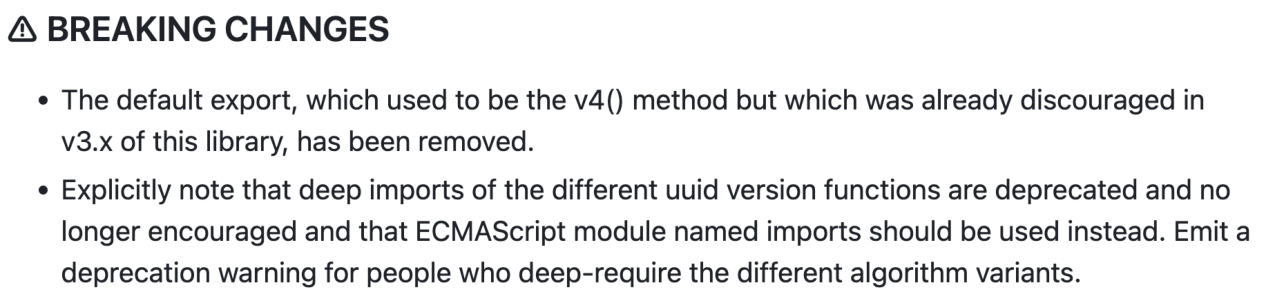
\includegraphics[width=0.9\linewidth]{BSthesis2024_Iida_fig/InsufficientDocumentation.pdf}}
\caption{uuidのバージョン7.0.0において公開された文書(CHANGELOG)の一部}
\label{fig:Insufficient_documentation}
\end{figure*}

\begin{figure*}[t]
\centerline{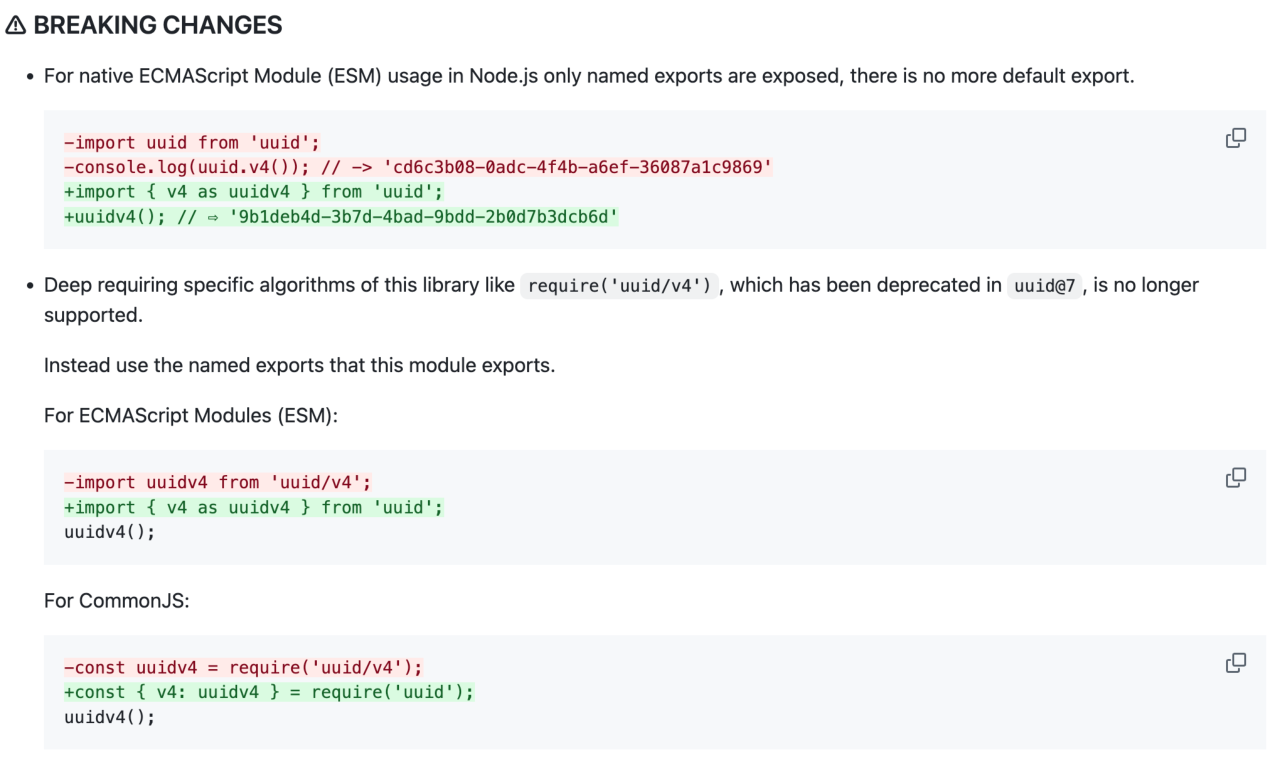
\includegraphics[width=0.9\linewidth]{BSthesis2024_Iida_fig/GoodDocumentation.pdf}}
\caption{uuidのバージョン8.0.0において公開された文書(CHANGELOG)の一部}
\label{fig:good_documentation}
\end{figure*}

\begin{figure*}[t]
\centerline{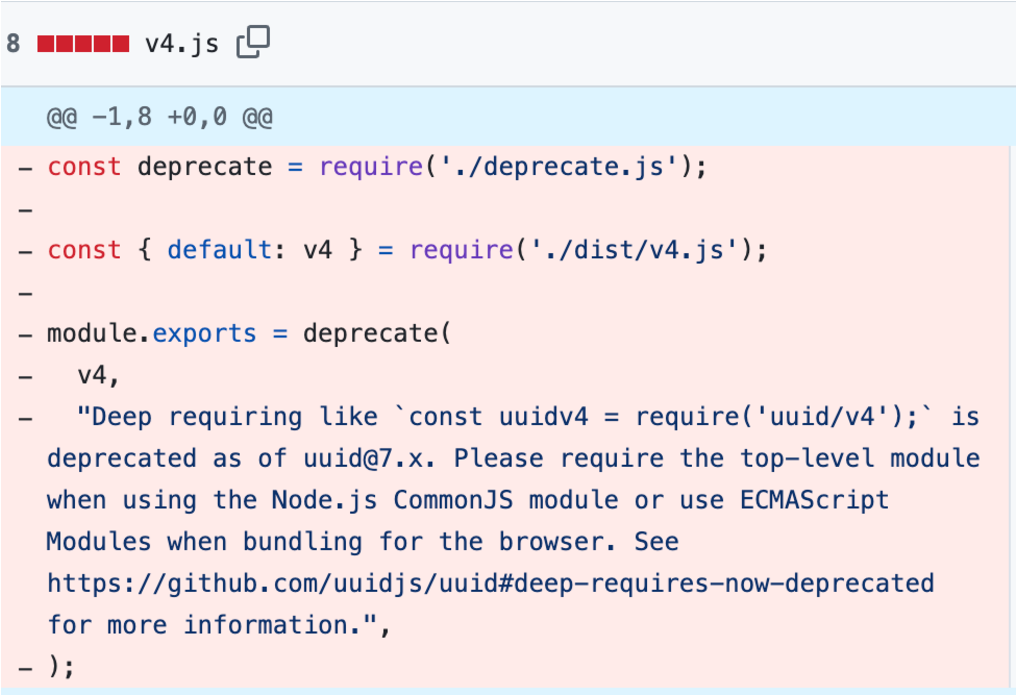
\includegraphics[width=0.75\linewidth]{@BSthesis2024_Iida/BSthesis2024_Iida_fig/uuid_library_code.pdf}}
\caption{uuidのバージョン7.0.3から8.0.0-beta.0への変更}
\label{fig:uuid_example}
\end{figure*}

%----------------------
\section{後方互換性の損失の課題}
ソフトウェア開発者はライブラリを利用することで効率的にソフトウェアを実装できるが,使用するライブラリのバージョン更新に後方互換性の損失が含まれるとクライアントが実行時エラーを引き起こすことがある.更新に後方互換性の損失を含む場合,クライアントは4種類の方法で対処を試みる\cite{DependedOnYou}.

\begin{itemize}
\item ライブラリのバージョンを正常に動作した更新前のバージョンにダウングレードする.
\item 実行時エラーの原因が修正されることを期待してアップグレードする.
\item 後方互換性の損失の影響を受けない実装方法に書き換える.
\item エラーが発生したライブラリが提供する機能の使用を停止する.
\end{itemize}

後方互換性の損失に影響を受けたクライアントが後方互換性の修正するためには,長い時間を要する\cite{DependedOnYou}.ここで,クライアント開発者が後方互換性の損失の影響を受けない実装方法に書き換える場合,実行時エラーが発生したプログラムの箇所と原因を特定する必要があるが,手作業で特定するのは困難である\cite{Nielsen2021JSFix}\cite{10.1145/3428255}.

後方互換性の損失を含むライブラリをリリースする場合,ライブラリ開発者は更新後の新しい実装方法を公開することもあるが,既存機能の変更内容に関する説明や変更前後の実装方法の例を提供しないような文書化が不十分な場合が存在する.
文書化が不十分な時,クライアントの開発者はライブラリの更新判断や修正にかけるコストが増加する\cite{mostafa2017experience}.ライブラリと公開される文書の例として,uuidライブラリの文書の一部を紹介する.図\ref{fig:Insufficient_documentation}はuuidのバージョン7.0.0において,後方互換性を損失した箇所の情報を説明文で公開した文書を示す.一方で,図\ref{fig:good_documentation}のuuidのバージョン8.0.0では後方互換性を損失した箇所に関する説明文,更新後にエラーとなる実装方法(赤色)と更新後に同じ振る舞いをする実装方法(緑色)を公開している.uuidのバージョン7.0.0のように説明文しか提供されない場合,クライアントは説明文から更新後にエラーとなる実装方法を理解し,更新判断や更新後に実行時エラーが発生する原因を特定しなければならない.


\section{従来研究}

ライブラリのバージョン更新における後方互換性の損失の有無を判定する手法としてテストを用いる手法が提案されている\cite{mujahid}\cite{matsuda}.Mujahidらは,ライブラリの後方互換性の損失の有無を判定するために,該当ライブラリに依存するクライアントのテストを用いた手法を提案している\cite{mujahid}.当該手法は,ライブラリのバージョン更新前後でクライアントのテストを実行し,成功していたテストがライブラリの更新後に失敗すれば後方互換性の損失と判定する.また,松田らは,ライブラリの機能の変更に伴うライブラリのテスト変更の有無から後方互換性の損失の有無を判定する手法を提案しており,クライアントのテスト結果をもとにした後方互換性の損失有無の判定を評価に利用している\cite{matsuda}.M{\o}llerらは,更新前のクライアントのテストをもとに更新前のAPIモデルを自動生成し,モデルを用いてバージョンX+1で動的解析することによりライブラリのAPIの型の変化を検知して後方互換性の損失を判定する手法を提案している\cite{10.1145/3338906.3338940}.本研究では,更新後にテストが失敗したクライアントのコードをもとに更新後にエラーとなる実装方法を正規表現を用いたパターンで表現する点が異なる.また,M{\o}llerらは,後方互換性の損失への対処を支援するために後方互換性の損失の影響を受けるクライアントのプログラムの場所を静的解析する手法を提案している\cite{10.1145/3428255}.この手法では,後方互換性の損失の影響を受けるパターン集を手作業で作成し,パターン集をもとにクライアントのソースコードを静的解析することで影響を受ける場所を検出している.ただし,後方互換性の損失の影響を受けるパターンの自動生成はしていない.


\section{動機}
ライブラリ開発者は,ライブラリ更新前後のクライアントの振る舞いを手作業により確認することで,後方互換性の損失によるクライアントへの影響範囲を特定できるかもしれない.しかし,ライブラリ更新のたびにクライアントのソースコードから使用方法を手作業で確認することはコストが膨大になるため現実的でない.

本研究では,事前分析としてライブラリのバージョン更新に伴って後方互換性の損失の影響を受けたクライアントがどのような実装方法で影響を受けたか調査した.JavaScriptライブラリであるuuidで後方互換性の損失を含む2種類のバージョン更新(uuid@7.0.3...8.0.0-beta.0,uuid@3.4.0...7.0.0-beta.0\footnote{本論文ではバージョン更新前後のバージョン名を「更新前バージョン名...更新後バージョン名」と記す.})のいずれかを実施し,テストが失敗したクライアントにおけるライブラリの実装方法を目視調査した.通常,ライブラリは\texttt{import}文または\texttt{require}文で定義されるライブラリ呼び出し文と関数呼び出し文の組を記述して使用される.
バージョン8.0.0-beta.0および7.0.0-beta.0の後方互換性の損失した変更内容の説明がWebサイトに公開されている\footnote{https://github.com/uuidjs/uuid/blob/v7.0.0/CHANGELOG.md}\footnote{https://github.com/uuidjs/uuid/blob/v8.0.0/CHANGELOG.md}.uuidのバージョン7.0.0-beta.0と8.0.0-beta.0はbeta版のバージョンであり,正式版バージョンの7.0.0と8.0.0の方で変更内容に関する文書が更新されていたため,正式版の文書を調査した.図\ref{fig:uuid_example}は,uuidライブラリの8.0.0-beta.0において後方互換性の損失を引き起こしたライブラリの変更であり,uuidのバージョン7.0.3から8.0.0への更新に伴い削除されたuuidライブラリのルートディレクトリに存在するファイルである.v4.jsファイルが削除されたことによりクライアントで図\ref{fig:good_documentation}下部の赤色(const uuidv4 = require('uuid/v4');)のようなライブラリの呼び出し文が使用できなくなっている.バージョン8.0.0では更新後にエラーとなる実装方法(赤色)を記載しているが,バージョン7.0.0では説明文のみで実装方法は記載されておらず,クライアントの対処を難しくする原因になっている.文書化されている変更内容は,クライアントでエラーを引き起こす実装方法の一部であった.例えば,7.0.0-beta.0において「\texttt{import * as uuid from 'uuid', uuid();}」の実装方法は使用できない呼び出し文であるが,文書で言及されていない.ライブラリの変更内容とバージョン更新後にテストが失敗したクライアントを調べると後方互換性の損失に影響を受ける実装方法は,ライブラリと関数呼び出し文の組で定義できると考えられる.そこで,テストが失敗したクライアントからライブラリと関数の呼び出し文を収集すれば,後方互換性の損失の影響を受ける実装方法を特定できるのではないかと考えた.ただし,クライアントにおける実装方法の例外も存在した.たとえば,キャッシュを経由して使用される場合やmock関数,「module.exports.\textless{}変数名\textgreater{}=\textless{}関数名\textgreater{}」のようにクライアントのファイル内でライブラリが提供する関数の名前を変えて使用する実装方法が挙げられる.こうした例外的なケースは追跡が困難であるため,本研究では,ライブラリの更新後にクライアントのテストが失敗したクライアントから,ライブラリと関数の呼び出し文に該当するのソースコード断片を抽出する.そして,後方互換性の損失の影響を受けるソースコード断片からライブラリと関数の呼び出し文の振る舞いに関係ない変数等を抽象化し,正規表現に変換した表現(\textbf{記述パターン})を自動生成する手法を提案する.さらに,提案する記述パターンによって後方互換性の損失の影響を受けるクライアントを特定する.本研究では,構文的な互換性と振る舞い的な互換性の両方を含むクライアントのテスト失敗を引き起こす後方互換性の損失を分析対象とする.

\section{リサーチクエスチョン}    
本研究では生成した記述パターンの有用性を評価するため,2つのリサーチクエスチョンを設定する.
\\
\noindent\textbf{RQ1:\RQOne}

本研究が提案する記述パターンが,後方互換性を損失するライブラリ開発者が把握している実装方法と把握していない実装方法の両方を生成できるかを確認する.具体的には,ライブラリが公開するリリースノート等の文書を確認し,記述パターンと同じ実装方法が明記されているかを調査する.文書に実装方法が明記されている場合にはライブラリ開発者が把握していると判断し,明記されてない場合に把握していない可能性があると考えられる.特に明記されていない実装方法を生成できれば,把握していない可能性のある実装方法を提供できるため,有用性が高いと考える.
\\
\noindent\textbf{RQ2:\RQTwo}

記述パターンは,更新後に使用するとエラーとなる実装方法のパターンである.そのため,記述パターンを持つクライアントは,後方互換性の損失の影響を受ける可能性が高い.テストが成功しているクライアントには,テストが不十分なためテストが成功する場合,後方互換性の損失に気づけていない可能性がある.そこで,テストが成功しているクライアントのうち,記述パターンを持つクライアントを検出することができれば,テストだけで気づけないクライアントに有用であると考える.そこで,バージョン更新後にテストが成功したクライアントでソースコードに記述パターンを含むクライアントを検出する.

%%%%%%%%%%%%%%%%%%%%%%%%%%%%%
\chapter{後方互換性の損失によるクライアントの特定手法}\label{sec:method}
%%%%%%%%%%%%%%%%%%%%%%%%%%%%%
%----------------------
\begin{figure*}[ht]
\centerline{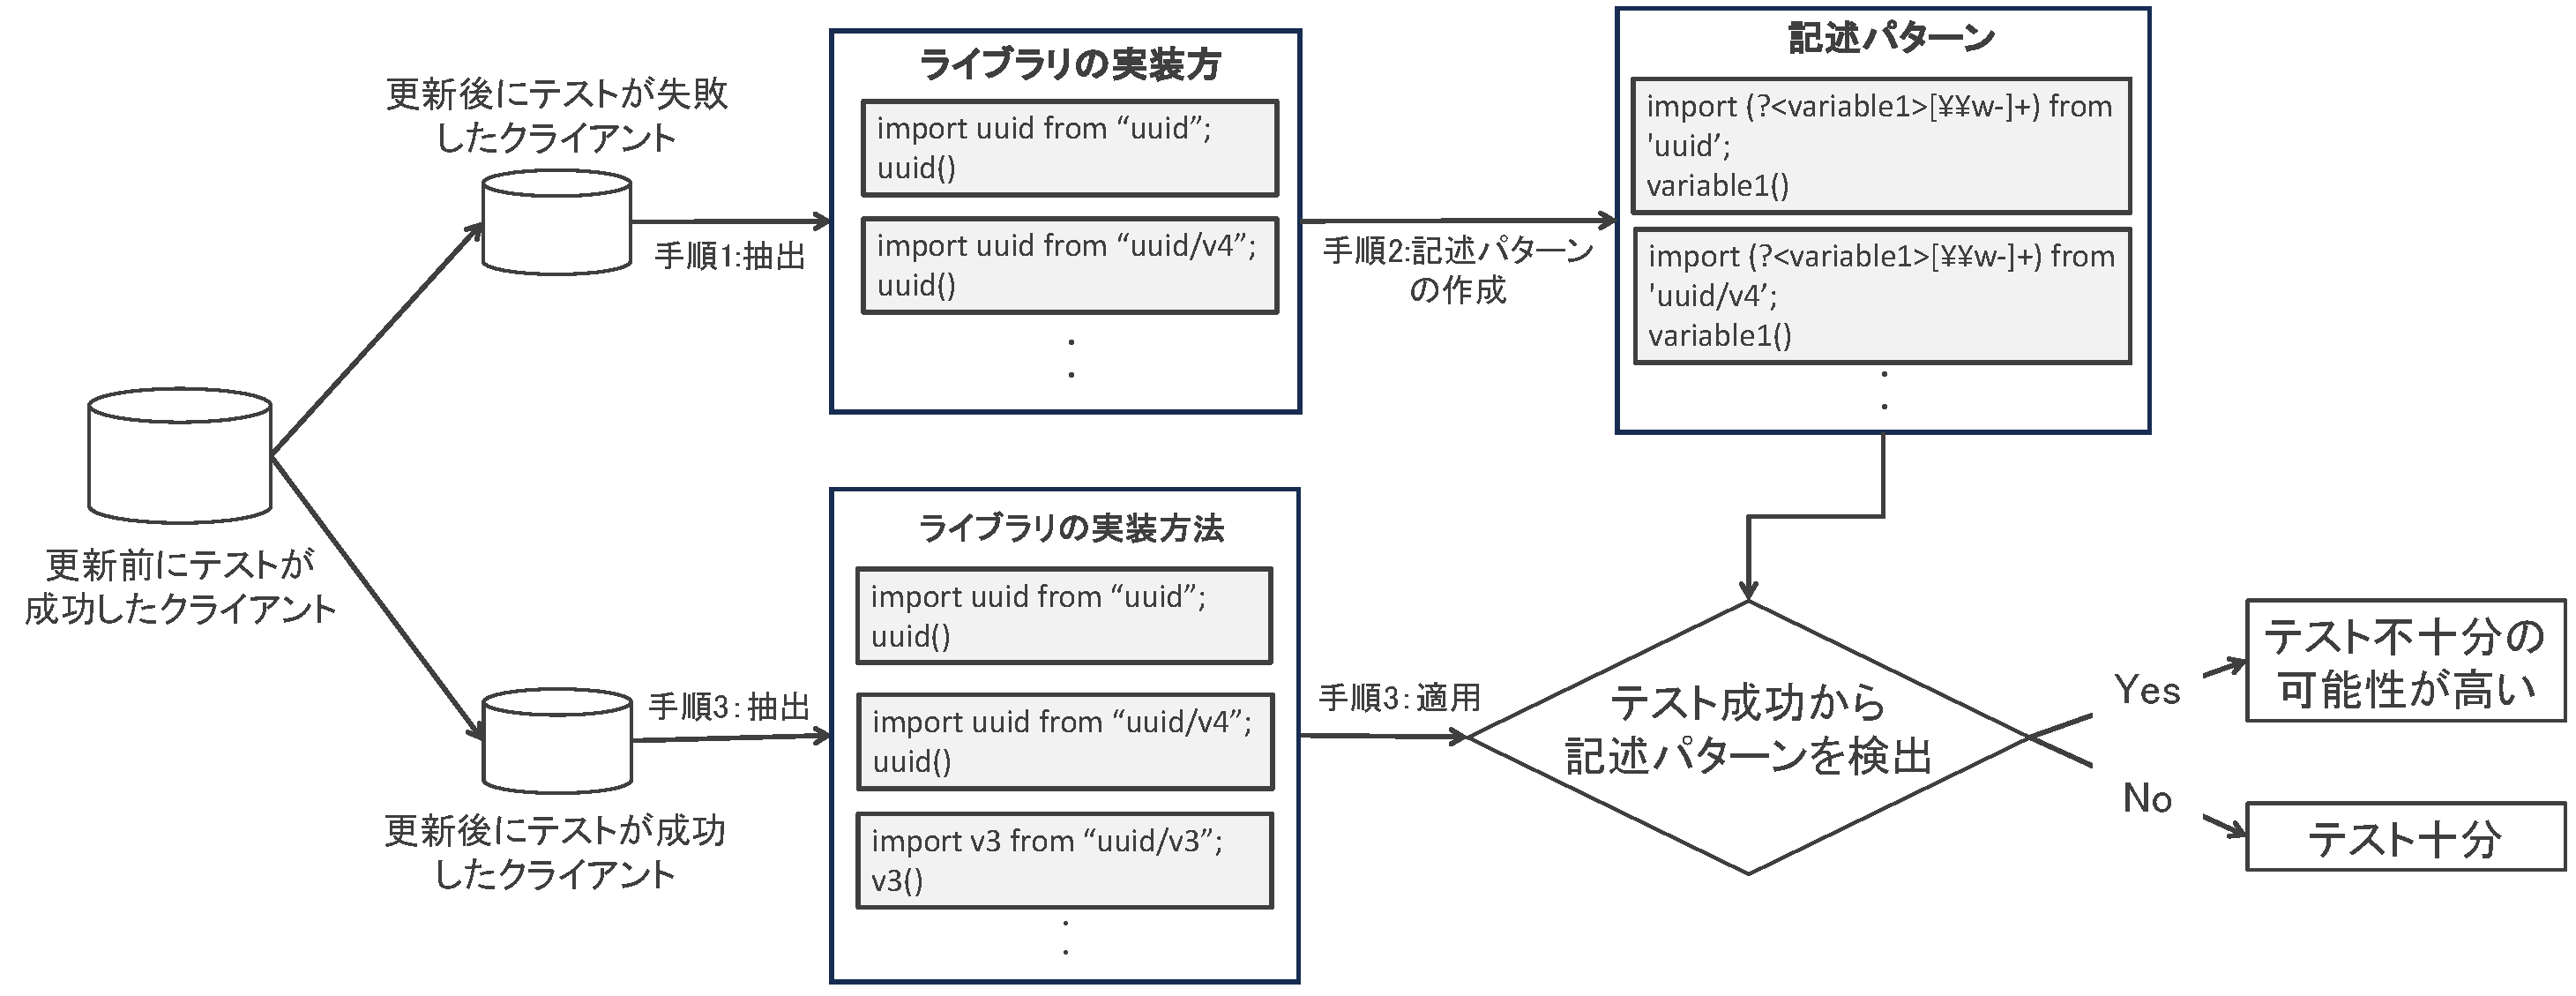
\includegraphics[width=1.0\linewidth]{BSthesis2024_Iida_fig/method.pdf}}
\caption{後方互換性の損失によるクライアントの特定手法の概略図}
\label{fig:method-overview}
\end{figure*}
%----------------------
\section{概要}
本章では,ライブラリの更新に伴いテストが失敗したクライアントから後方互換性の損失の影響を受ける呼び出し文,および関数呼び出し文の記述パターンを自動生成する手法を述べる.本研究の記述パターンとは,ライブラリのバージョン更新後にエラーとなる実装方法を指す.クライアントのテストは,ライブラリを使用するクライアントの開発者が単体テストや結合テストのために準備したテストケースを指し,ライブラリのバージョン更新前後でクライアントのテスト結果が成功から失敗に変わったものを「テストが失敗」と定義し,後方互換性の損失による影響を検出できたことがわかる.一方で,テスト失敗以外のクライアントを「テストが成功」と定義し,後方互換性の損失の影響を受けなかったまたは検出漏れの可能性が示唆される.前提条件としてクライアントのテスト結果は,従来研究\cite{matsuda}の筆者らがクライアントが使用していたライブラリのバージョンを1つずつ更新しながらテストした結果である.図\ref{fig:method-overview}に後方互換性の損失によるクライアントの特定手法の概略図を示し,各手順を説明をする.

\section{記述パターンの生成方法}

\subsection{手順1.テストが失敗したクライアントからライブラリの呼び出し文,関数呼び出し文を抽出}
ライブラリは,ライブラリの呼び出し文と関数呼び出し文を用いてクライアントで使用される.本研究で分析対象とするJavaScriptとTypeScriptにおいてライブラリの呼び出し文は\texttt{import}文または\texttt{require}文で定義され,関数呼び出し文はライブラリ呼び出し文でクライアントが定義した変数名をもとに定義されている.そのため,ライブラリの呼び出し文は,クライアントのJavaScriptとTypeScriptのソースファイルに正規表現を用いて\texttt{import}文または\texttt{require}文を持ち,ライブラリ名を定義しているという条件を満たす行を抽出する.この時,関数呼び出し文の抽出に向けてライブラリ呼び出し文で定義される変数名(例:「import id from 'uuid'」の場合,変数名は「id」)も同時に取得する.次にライブラリが使用されていたファイル内のソースコードを抽象構文木に変換し,変数名をもとに使用されているライブラリの関数呼び出し文を抽出する.抽象構文木に変換する理由は,引数の定義方法や関数の定義方法によって正規表現で取得することに限界があるためである.抽象構文木に変換することで関数として使用される部分をノードごとに判別して取得することができ,誤抽出を低下させることができる.ここで,クライアントに抽象構文木を作成できないファイルがあるとライブラリと関数の呼び出し文を抽出できない可能性があるため,全てのJavaScriptとTypeScriptのファイルから抽象構文木を生成できるクライアントだけをパターン生成に使用している.

\subsection{手順2.ライブラリ呼び出し文,関数呼び出し文による記述パターンの自動生成}
%-----------------------
\begin{table}[t]
\centering
\caption{記述パターンの生成例}
\label{table:abstractionsample}
\scalebox{0.9}{
    \begin{tabular}{l|l}
    \hline 
        変換前 & 変換後 \\ \hline \hline
        \begin{tabular}[c]{@{}l@{}}\texttt{import uuid from 'uuid'}\\ \texttt{uuid()}\end{tabular} &
        \begin{tabular}[c]{@{}l@{}}\texttt{import (?\textless{}variable1\textgreater{}{[}\textbackslash{}w-{]}+) from ["'\`{}]uuid["'\`{}][\^{}.]*}\\ \texttt{variable1()[\^{}.]*}\end{tabular} \\ \hline
        \begin{tabular}[c]{@{}l@{}}\texttt{import v4 from `uuid/v4'}\\ \texttt{v4}();\end{tabular} & 
        \begin{tabular}[c]{@{}l@{}}\texttt{import (?\textless{}variable1\textgreater{}{[}\textbackslash{}w-{]}+) from ["'\`{}]uuid/v4["'\`{}][\^{}.]*}\\ \texttt{variable1()[\^{}.]*}\end{tabular} \\ \hline
        \begin{tabular}[c]{@{}l@{}}\texttt{import uuid from "uuid"}\\ \texttt{uuid.v4()}\end{tabular} & \begin{tabular}[c]{@{}l@{}}\texttt{import (?\textless{}variable1\textgreater{}{[}\textbackslash{}w-{]}+) from ["'\`{}]uuid["'\`{}][\^{}.]*}\\ \texttt{variable1.v4()[\^{}.]*}\end{tabular} \\ \hline
    \end{tabular}
}
\end{table}
%-----------------------

ライブラリ呼び出し文,関数呼び出し文の変数名の部分は,クライアントが自由に設定できる部分であるため抽象化したのち,正規表現として記述パターンを生成する.具体的には,図\ref{fig:method-overview}における記述パターンの生成では,ライブラリと関数呼び出し文を表\ref{table:abstractionsample}のように変換する.ライブラリ呼び出し文,関数呼び出し文において,各クライアントが命名した変数名は表\ref{table:abstractionsample}の\texttt{variable}のように抽象化して表現する.抽象化後にライブラリの呼び出し文とライブラリの関数呼び出し文を紐づけるため,抽象化した名前に図\ref{fig:method-overview}の\texttt{variable1}のようなIDを付与し,1つのクライアントで共通する変数名を紐づける.ただし,「\texttt{import \{v4\} from 'uuid'}」の「\texttt{\{v4\}}」のように指定されている場合は,変数名がライブラリの関数を表すため,変数名を抽象化しない.改行のような特殊文字や記述パターンの前後の空白は,ライブラリに関する実装方法に関係ないため削除する.モック関数や「module.exports.id=uuid」(idの箇所は任意の文字列)のような実装方法をしているクライアントは関数呼び出し文が特殊になるため,除外している.生成した記述パターンにおいて包含関係のあるパターン対が存在する場合があるため,自動的に記述パターンの集約を行う.パターンの集約では,すべてのパターン間で相互にマッチングを行い,より広く適用可能なパターンを残すため,誤検出や取りこぼしが発生するリスクはない.

ライブラリ関数の引数がクライアントで定義されている場合には,引数の中身は保持せず引数の数のみを確認するように記述パターンを変換する.本研究において各クライアントが命名した変数名の影響を抽象化によって取り除いているため引数の数を正確に取得できるが,引数が変数としてまとめられている場合には引数の数を正確に取得できない.しかし,ライブラリ開発者は,誤った記述パターンを提示された際に誤りの有無を判別できると考えられるため,
検出する再現率が向上するように抽象度の高い記述パターンを生成する.抽象度を高くするため,ライブラリの振る舞いに関係しない箇所の条件を緩くするため,以下のような工夫をしている.

\begin{itemize}
\item 「'」,「"」,「`」の違いを許容するために["'\`{}]の正規表現に置換する.
\item 「let」,「const」,「var」を削除する.
\item コードの末尾につく「;」を削除する.ただし,「;」を除外した場合にライブラリ呼び出し文の末尾に「.\textless{}関数名\textgreater{}」が記述される場合に誤検出することがあるため,記述パターンの末尾に「.」が存在する場合にはマッチングしないように条件を追加し,対策している.
\end{itemize}

フィルタリング,抽出,抽象化を含む処理をテストに失敗したクライアントのリポジトリごとに行い,クライアントが記述しているライブラリに関する全ての実装方法をまとめることで記述パターンを生成する.ただし,ライブラリ呼び出し単体しか記述パターンを抽出できなかったクライアントは,特殊な呼び出し文である可能性が高いためクライアントごと除外する.
\section{記述パターンによる検出方法}

\subsection{手順3.クライアントのテストが成功する中で後方互換性の損失による影響を受けるクライアントの検出}

後方互換性の損失の影響を受けたクライアントから生成した記述パターンを用いて,テストが成功しているクライアントが後方互換性の損失の影響を受けたクライアントと同じ実装で記述しているクライアントを検出する.具体的に,手順1のようにテストが成功したクライアントからライブラリの呼び出し文と関数呼び出し文を抽出する.次に記述パターンを適用し,クライアントの\texttt{import}や\texttt{require}から始まるライブラリの呼び出し文を検出する.ここで,ライブラリの呼び出し文が一致した場合には変数名の部分を取得し,記述パターンの中で対応する関数呼び出し文の同じ変数名の部分をクライアントが設定していた変数名に置換する.続いて関数呼び出し文もライブラリ呼び出し文と同様に,テストが成功しているクライアントの中から後方互換性の損失の影響を受ける関数呼び出し文の記述を用いているクライアントを検出する.クライアントの実装方法が記述パターンに含まれるライブラリ呼び出し文と関数呼び出し文の両方に完全一致すれば,該当クライアントが後方互換性の損失の影響を受けているが,テスト不十分により気づいていなかったクライアントである可能性が高いと判定する.


%%%%%%%%%%%%%%%%%%%%%%%%%%%%%
\chapter{ケーススタディ}\label{chap:case_study}
%%%%%%%%%%%%%%%%%%%%%%%%%%%%%
\section{データセット}
%%%%%%%%%%%%%%%%%%%%%%%%%%%%%
\begin{table}[b]
    \caption{分析対象としたライブラリ}
    \label{table:dataset}
    \centering
    \scalebox{1.0}{
        \begin{tabular}{l|r|r|r}
        \hline 
        \begin{tabular}{c} ライブラリ名@旧バージョン{...}\\新バージョン \end{tabular}&  \begin{tabular}{c}更新前の\\テスト成功 \end{tabular}&  \begin{tabular}{c}更新後の\\テスト失敗 \end{tabular}&  \begin{tabular}{c}更新後の\\テスト成功 \end{tabular}\\ \hline \hline
        uuid@7.0.3...8.0.0-beta.0 & 433 & 119 & 314 \\
        uuid@3.4.0...7.0.0-beta.0 & 490 & 55 & 435 \\
        globby@8.0.0...8.0.1 & 128 & 42 & 86 \\
        meow@3.6.0...4.0.0 & 154 & 26 & 128 \\
        globby@6.1.0...7.0.0 & 137 & 24 & 113 \\
        pump@1.0.3...2.0.0 & 102 & 19 & 83 \\
        globby@7.1.1...8.0.0 & 143 & 16 & 127 \\
        vinyl@1.2.0...2.0.0 & 69 & 11 & 58 \\
        \hline
        \end{tabular}
    }
\end{table}
%%%%%%%%%%%%%%%%%%%%%%%%%%%%%
本研究では,従来研究においてMujahidらが公開するデータセットを分析対象とする.データセットには,GitHubリポジトリが記載されている,未成熟なクライアントを除外するためにライブラリを記述するファイル(package.json)の変更履歴が2回以上存在する.290,417件のJavaScriptライブラリと各ライブラリのいずれかのバージョンに依存するクライアントのリポジトリやコミットIDなどの情報が含まれている.このデータセットの中から,従来研究\cite{matsuda}が3つの条件で抽出した238件のJavaScriptライブラリとバージョンの2,111組のライブラリのバージョン,各ライブラリのバージョンのクライアントのテスト実行結果を用いる.各条件は次に示す.

\begin{itemize}
\item ライブラリにテストが付属していること
\item ライブラリの人気度合いを示すnpmスコア\footnote{\url{https://npms.io}}が上位500件以内であること
\item バージョンがリリースされた変更のコミットステータス\footnote{\url{https://www.npmjs.com/}}からテスト結果を確認し,テスト実行時の成功率が 100\%であること
\end{itemize}

本研究が定義する後方互換性を損失するライブラリのバージョンは,従来研究\cite{mujahid}と同様に,ライブラリのバージョンを使用するクライアントが保有するテストケースの中が1件以上失敗していることを条件とする.本研究が提案する手法は,テストが失敗するクライアントが少ない場合,後方互換性が損失するライブラリと関数呼び出し文をもとにした記述パターンを生成できない可能性があるため,従来研究\cite{matsuda}が分析対象とする2,111組のライブラリのバージョンの中で,さらに次の2つの条件を満たした8組を分析対象とする.
\begin{itemize}
\item 10件以上クライアントがテストに失敗しているライブラリのバージョン
\item 50件以上のクライアントがテストに成功しているライブラリのバージョン
\end{itemize}
表\ref{table:dataset}は,本研究で分析対象とする8組のライブラリのバージョン,およびライブラリ旧バージョンでテストが成功したクライアント数,ライブラリ新バージョン適用後のテスト結果を示す.

%%%%%%%%%%%%%%%%%%%%%%%%%%%%%
\section{RQ1:\RQOne}\label{sec:RQ1}

%%%%%%%%%%%%%%%%%%%%%%%%%%%%%

\begin{table*}[t]
     \caption{記述パターンを取得できたクライアント数}
     \label{table:RQ1}
    \centering
     \scalebox{0.65}{
         \begin{tabular}{l|r|r|r|r}
         \hline 
         \begin{tabular}{c} ライブラリ名@旧バージョン{...}\\新バージョン \end{tabular}
         & \begin{tabular}{c} テスト失敗\\クライアント数 \end{tabular}
         & \begin{tabular}{c} 記述パターン候補 \end{tabular}
         & \begin{tabular}{c}集約後の\\記述パターン種類数\end{tabular}
         & \begin{tabular}{c} テスト成功の検出時に\\使用された記述パターン種類数 \end{tabular}
         \\ \hline \hline
         uuid@7.0.3...8.0.0-beta.0 & 119 & 100 & 9 & 4\\
         uuid@3.4.0...7.0.0-beta.0 & 55 & 43  & 11 & 7\\
         globby@8.0.0...8.0.1 & 42 & 31 & 10 & 6\\
         meow@3.6.0...4.0.0  & 26 & 17 & 5 & 3\\
         globby@6.1.0...7.0.0 & 24 & 19 & 7 & 6\\
         pump@1.0.3...2.0.0 & 19 & 17 & 2 & 1\\
         globby@7.1.1...8.0.0 & 16 & 15 & 5 & 5\\
         vinyl@1.2.0...2.0.0  & 11 & 10 & 2 & 1\\
         \hline
         \end{tabular}
         }
\end{table*}
%%%%%%%%%%%%%%%%%%%%%%%%%%%%%

\subsection{実験結果}
\noindent\textbf{1.記述パターンを生成した結果}

表\ref{table:RQ1}は,テストに失敗したクライアントのライブラリ呼び出し文,関数呼び出し文から生成した記述パターンの種類数を示す.例としてuuid@7.0.3...8.0.0-beta.0では,バージョン更新後にテストが失敗したクライアントである119件のうち,100件のクライアントで記述パターン候補を生成することができた.残り19件のクライアントは,JavaScriptまたはTypeScriptで記述されたファイルに対して抽象構文木が作成できない場合やクライアントから抽出できたソースコード断片がライブラリ呼び出し文のみである場合にクライアントから全ての呼び出し文を抽出することができない可能性があるため除外した.100件の記述パターン候補には包含関係を持つ場合が存在する.それらに対して包含関係として広く検出できる記述パターン候補を残す形で集約を行い,最終的に記述パターン数は9件となった.このような処理を各ライブラリのバージョンにおけるクライアントに行なった結果,本研究で分析対象とした8組のライブラリのバージョンにおいて,2種類から11種類の集約した記述パターンを生成できた.

\textbf{\newline\newline}
\noindent\textbf{2.記述パターンがライブラリに記載がある後方互換性を損失する実装方法を表現できているかの調査結果}

%----------------------
% \begin{table*}[t]
% \centering
% \caption{バージョン更新に伴い変更された文書}
% \label{table:note}
% \scalebox{0.9}{
%     \begin{tabular}{l|c|c}
%         \hline
%         \begin{tabular}{c}ライブラリ名@旧バージョン{...}\\新バージョン\end{tabular} &\begin{tabular}{c}文書あり/なし(記述先)\end{tabular}& \begin{tabular}{c}説明文あり/なし(記述先)\end{tabular} \\ \hline \hline
%         uuid@7.0.3...8.0.0-beta.0 & 文書あり(CHANGELOG\footnote{\url{https://github.com/uuidjs/uuid/blob/v8.0.0/CHANGELOG.md}}) & 説明文あり(CHANGELOG) \\ \hline
%         uuid@3.4.0...7.0.0-beta.0 & 文書なし & 説明文あり(CHANGELOG\footnote{\url{https://github.com/uuidjs/uuid/blob/v7.0.0/CHANGELOG.md}}) \\ \hline
%         globby@8.0.0...8.0.1 & 文書なし & 説明文なし \\ \hline
%         meow@3.6.0...4.0.0 & 文書あり(リリースノート\footnote{\url{https://github.com/sindresorhus/meow/releases/tag/v4.0.0/}}) & 説明文あり(リリースノート) \\ \hline
%         globby@6.1.0...7.0.0 & 文書なし & 説明文あり(リリースノート\footnote{\url{https://github.com/sindresorhus/globby/releases/tag/v7.0.0/}}) \\ \hline
%         pump@1.0.3...2.0.0 & 文書なし & 説明文なし \\ \hline
%         globby@7.1.1...8.0.0 & 文書なし & 説明文あり(リリースノート\footnote{\url{https://github.com/sindresorhus/globby/releases/tag/v8.0.0/}}) \\ \hline
%         vinyl@1.2.0...2.0.0 & 文書なし & 説明文あり(リリースノート\footnote{\url{https://github.com/gulpjs/vinyl/releases/tag/v2.0.0}}) \\ \hline
%     \end{tabular}
% }
% \end{table*}
\begin{table*}[t]
\centering
\caption{バージョン更新に伴い変更された文書}
\label{table:note}
\scalebox{0.9}{
    \begin{tabular}{l|c|c}
        \hline
        \begin{tabular}{c}ライブラリ名@旧バージョン{...}\\新バージョン\end{tabular} & \begin{tabular}{c}説明文あり/なし(記述先)\end{tabular} & \begin{tabular}{c}文書あり/なし(記述先)\end{tabular} \\ \hline \hline
        uuid@7.0.3...8.0.0-beta.0 & 説明文あり(CHANGELOG\footnote{\url{https://github.com/uuidjs/uuid/blob/v8.0.0/CHANGELOG.md}}) & 文書あり(CHANGELOG) \\ \hline
        uuid@3.4.0...7.0.0-beta.0 & 説明文あり(CHANGELOG\footnote{\url{https://github.com/uuidjs/uuid/blob/v7.0.0/CHANGELOG.md}}) & 文書なし \\ \hline
        globby@8.0.0...8.0.1 & 説明文なし & 文書なし \\ \hline
        meow@3.6.0...4.0.0 & 説明文あり(リリースノート\footnote{\url{https://github.com/sindresorhus/meow/releases/tag/v4.0.0/}}) & 文書あり(リリースノート) \\ \hline
        globby@6.1.0...7.0.0 & 説明文あり(リリースノート\footnote{\url{https://github.com/sindresorhus/globby/releases/tag/v7.0.0/}}) & 文書なし \\ \hline
        pump@1.0.3...2.0.0 & 説明文なし & 文書なし \\ \hline
        globby@7.1.1...8.0.0 & 説明文あり(リリースノート\footnote{\url{https://github.com/sindresorhus/globby/releases/tag/v8.0.0/}}) & 文書なし \\ \hline
        vinyl@1.2.0...2.0.0 & 説明文あり(リリースノート\footnote{\url{https://github.com/gulpjs/vinyl/releases/tag/v2.0.0}}) & 文書なし \\ \hline
    \end{tabular}
}
\end{table*}

% \footnotetext[1]{\url{https://github.com/uuidjs/uuid/blob/v8.0.0/CHANGELOG.md}}
% \footnotetext[2]{\url{https://github.com/uuidjs/uuid/blob/v7.0.0/CHANGELOG.md}}
% \footnotetext[3]{\url{https://github.com/sindresorhus/meow/releases/tag/v4.0.0/}}
% \footnotetext[4]{\url{https://github.com/sindresorhus/globby/releases/tag/v7.0.0/}}
% \footnotetext[5]{\url{https://github.com/sindresorhus/globby/releases/tag/v8.0.0/}}
% \footnotetext[6]{\url{https://github.com/gulpjs/vinyl/releases/tag/v2.0.0}}
%----------------------
% \begin{table*}[t]
% \centering
% \caption{バージョン更新に伴い変更された文書}
% \label{table:note}
% \scalebox{0.9}{
%     \begin{tabular}{l|l|l|l}
%         \hline
%         \begin{tabular}{c}ライブラリ名@旧バージョン{...}\\新バージョン\end{tabular} & \begin{tabular}{c}更新された文書\end{tabular} & \begin{tabular}{c}リリースノート\end{tabular} & \begin{tabular}{c}変更内容の記載文書\end{tabular} \\ \hline \hline
        
%         uuid@7.0.3...8.0.0-beta.0 & \begin{tabular} {l}CHANGELOG\\README\\README\_js \end{tabular}& 文章なし & CHANGELOG \\ \hline
%         uuid@3.4.0...7.0.0-beta.0 & \begin{tabular} {l}CHANGELOG\\README\\README\_js \end{tabular}& 文章なし & CHANGELOG \\ \hline
%         globby@8.0.0...8.0.1 & なし & 文章なし & なし \\ \hline
%         meow@3.6.0...4.0.0 & README & \textbf{文章あり} & リリースノート \\ \hline
%         globby@6.1.0...7.0.0 & README & \textbf{文章あり} & リリースノート \\ \hline
%         pump@1.0.3...2.0.0 & なし & 文章なし & なし \\ \hline
%         globby@7.1.1...8.0.0 & README & \textbf{文章あり} & リリースノート \\ \hline
%         vinyl@1.2.0...2.0.0 & README & \textbf{文章あり\footnotemark} & リリースノート \\ \hline
%     \end{tabular}
% }
% \end{table*}
%----------------------
\begin{figure*}[t]
\centerline{\includegraphics[width=0.9\linewidth]{@BSthesis2024_Iida/BSthesis2024_Iida_fig/RQ1_bar_graph.pdf}}
\caption{生成した記述パターンと文書化の有無を表した棒グラフ}
\label{fig:bar_plot}
\end{figure*}
%----------------------

%/は\textbackslash  < \textless{} > \textgreater{}
\begin{table}[t]
    \caption{uuid@7.0.3...8.0.0-beta.0の記述パターン}
    \label{table:uuid8.0.0_description pattern}
    \centering
    \scalebox{0.80}{
        \begin{tabular}{c|l|c|r}
        \hline
            ID & \begin{tabular}{c}記述パターン(上はライブラリ呼び出し文,下は時間数呼び出し文)\end{tabular}&  \begin{tabular}{c}文書\\あり/なし\end{tabular} & \begin{tabular}{c}全クライアント\\での検出数\end{tabular} \\ \hline
            \hline 
        
            \multirow{2}{*}{1} & \texttt{(?\textless{}variable1\textgreater{}{[}\textbackslash{}w-{]}+) = require(["'\`{}]uuid/v4["'\`{}])[\^{}.]*} & \multirow{2}{*}{あり} & \multirow{2}{*}{84/433}\\ \cline{2-2}
            & \texttt{variable1()[\^{}.]*} & & \\ \hline

            \multirow{2}{*}{2} & \texttt{(?\textless{}variable1\textgreater{}{[}\textbackslash{}w-{]}+) = require(["'\`{}]uuid/v1["'\`{}])[\^{}.]*} & \multirow{2}{*}{あり} & \multirow{2}{*}{26/433} \\ \cline{2-2}
            & \texttt{variable1()[\^{}.]*} & & \\ \hline

            \multirow{2}{*}{3} & \texttt{import (?\textless{}variable1\textgreater{}{[}\textbackslash{}w-{]}+) from ["'\`{}]uuid/v4["'\`{}][\^{}.]*} & \multirow{2}{*}{あり} & \multirow{2}{*}{21/433} \\ \cline{2-2}
            & \texttt{variable1()[\^{}.]*} & & \\ \hline

            \multirow{2}{*}{4} & \texttt{import (?\textless{}variable1\textgreater{}{[}\textbackslash{}w-{]}+) from ["'\`{}]uuid/v1["'\`{}][\^{}.]*} & \multirow{2}{*}{あり} & \multirow{2}{*}{5/433}  \\ \cline{2-2}
            & \texttt{variable1()[\^{}.]*} & & \\ \hline 
            
            \multirow{2}{*}{5} & \texttt{import * as (?\textless{}variable1\textgreater{}{[}\textbackslash{}w-{]}+) from ["'\`{}]uuid/v4["'\`{}][\^{}.]*} & \multirow{2}{*}{なし}  &  \multirow{2}{*}{5/433} \\ \cline{2-2}
            & \texttt{variable1()[\^{}.]*} & & \\ \hline
            
            \multirow{2}{*}{6} & \texttt{import * as (?\textless{}variable1\textgreater{}{[}\textbackslash{}w-{]}+) from ["'\`{}]uuid/v1["'\`{}][\^{}.]*} & \multirow{2}{*}{なし}  &  \multirow{2}{*}{4/433} \\ \cline{2-2}
            & \texttt{variable1()[\^{}.]*} & & \\ \hline
            
            \multirow{2}{*}{7} & \texttt{(?\textless{}variable1\textgreater{}{[}\textbackslash{}w-{]}+) = require(["'\`{}]uuid/v4["'\`{}] )[\^{}.]*} & \multirow{2}{*}{あり} & \multirow{2}{*}{1/433}  \\ \cline{2-2}
            & \texttt{variable1([\textasciicircum,]*,[\textasciicircum,]*,[\textasciicircum,]*)[\^{}.]*} & & \\ \hline
            
            \multirow{4}{*}{8} & \texttt{(?\textless{}variable1\textgreater{}{[}\textbackslash{}w-{]}+) = require(["'\`{}]uuid/v4["'\`{}])[\^{}.]*} & \multirow{4}{*}{なし} & \multirow{4}{*}{1/433}  \\
            & \texttt{import * as (?\textless{}variable1\textgreater{}{[}\textbackslash{}w-{]}+) from ["'\`{}]uuid/v4["'\`{}][\^{}.]*} & & \\ \cline{2-2}
            & \texttt{variable1([\textasciicircum,]*,[\textasciicircum,]*)[\^{}.]*}& & \\ 
            & \texttt{variable2([\textasciicircum,]*,[\textasciicircum,]*)[\^{}.]*}& & \\ \hline
            
            \multirow{7}{*}{9} & \texttt{(?\textless{}variable1\textgreater{}{[}\textbackslash{}w-{]}+) = require(["'\`{}]uuid["'\`{}])[\^{}.]*} & \multirow{7}{*}{あり} & \multirow{7}{*}{1/433} \\ 
            & \texttt{(?\textless{}variable2\textgreater{}{[}\textbackslash{}w-{]}+) = require(["'\`{}]uuid/v1["'\`{}])[\^{}.]*} & & \\
            & \texttt{(?\textless{}variable3\textgreater{}{[}\textbackslash{}w-{]}+) = require(["'\`{}]uuid/v4["'\`{}])[\^{}.]*} & & \\
            & \texttt{(?\textless{}variable4\textgreater{}{[}\textbackslash{}w-{]}+) = require(["'\`{}]uuid/v5["'\`{}])[\^{}.]*} & & \\ \cline{2-2}
            
            & \texttt{variable2.apply([\textasciicircum,]*,[\textasciicircum,]*)[\^{}.]*}& & \\ 
            & \texttt{variable3.apply([\textasciicircum,]*,[\textasciicircum,]*)[\^{}.]*}& & \\
            & \texttt{variable4.apply([\textasciicircum,]*,[\textasciicircum,]*)[\^{}.]*}& & \\ \hline
        \end{tabular}
    }
\end{table}

%----------------------

%%%%%%%%%%%%%%%%%%%%%%%%%%%%%

本研究で生成した記述パターンの有用性を確かめるためにライブラリがバージョンをリリースする際に公開するリリースノートやCHANGELOG,READMEなどの文書を目視調査した.具体的には,後方互換性の損失に関する説明文が存在しているか,生成した記述パターンと同じ意味を持つ後方互換性を損失する実装方法がライブラリのリリース時に公開された文書に記載されているかの2点を調べる.uuidの2つのバージョン(7.0.0-beta.0と8.0.0-beta.0)に関しては,beta版であるため文書が整備されていない可能性を考慮し,beta版の後にリリースされた正式版(バージョン7.0.0とバージョン8.0.0)の文書を調査している.beta版と正式版uuidの(7.0.0-beta.0と7.0.0
\footnote{\url{https://github.com/uuidjs/uuid/compare/522e44c055871493303ec0158dac75d7ce1eba5b...63e5702d7629303a5193c4dd31825376f240f888}},8.0.0-beta.0と8.0.0
\footnote{\url{https://github.com/uuidjs/uuid/compare/99d65afdc42b98377842756c0743bc38dcb03570...a7d3d517382490eda6dd21158e5413261c45ccdd}})の間でテストの更新や文書の追加のみが行われ,beta版からの機能変更が存在しないことを確認している.表\ref{table:note}は,バージョン更新に伴い更新された文書と変更内容が記載された文書を調べた結果である.左から順にライブラリ名とバージョン,後方互換性の損失に関する説明文の有無,後方互換性を損失する実装方法に関する文書の有無を示している. 表\ref{table:note}の2列目より8組中6組では,後方互換性の損失に関わる変更内容の説明文が記載されている.また,3列目よりuuidのバージョン8.0.0-beta.0とmeowのバージョン4.0.0の2組のみで後方互換性を損失する実装方法を記載していた.後方互換性を損失する実装方法が記載されていたuuidのCHANGELOGとmeowのリリースノートと生成した記述パターンを比較した結果,ライブラリの文書に記載されていた実装方法を記述パターンによって表現できていることを確認できた.

\textbf{\newline\newline}
\noindent\textbf{3.ライブラリに文書化されていない記述パターンの調査結果}

記述パターンの一部は,各ライブラリが周知する後方互換性を損失する実装方法に含まれていない.図\ref{fig:bar_plot}は,各ライブラリのバージョン更新時に記述パターンと同じ意味を持つ実装方法が文書化されているか否かを表した棒グラフで,横軸がライブラリのバージョン,縦軸が記述パターン数を表す.棒グラフの白色の部分は,ライブラリに文書化されていなかった記述パターンを表し,黒い部分は文書化されていた記述パターンを表している.図\ref{fig:bar_plot}よりmeowライブラリとuuidライブラリの2組では,生成した記述パターンと同じ意味を持つ実装方法が後方互換性を損失する実装方法として大部分が記載されていた.一方で,他の6組のライブラリでは記述パターンのような実装方法が文書に記載されていなかった.記述パターンはライブラリで文書化されている後方互換性を損失する実装方法を正しく生成できるだけでなく,周知されていない実装方法の生成も可能であることを確認できた.具体的な例としてuuidライブラリのバージョン8.0.0-beta.0で生成した記述パターンの一覧とライブラリが周知する後方互換性を損失する実装方法として記載があるかを調査した結果を表\ref{table:uuid8.0.0_description pattern}に示す.各列は,ID,記述パターン(上部にライブラリ呼び出し文,下部に関数呼び出し文),ライブラリ文書に後方互換性を損失する実装方法として記載されているか否か,テストを成功または失敗したクライアントの全体で記述パターンを用いて検出できたクライアント数を表す.表\ref{table:uuid8.0.0_description pattern}のID5,ID6,ID8の記述パターンがライブラリのCHANGELOG\footnote{\url{https://github.com/uuidjs/uuid/blob/v8.0.0/CHANGELOG.md}}で周知されていない実装方法であり,図\ref{fig:bar_plot}の最も右側にあるグラフの黒色に対応している.このように,記述パターンは後方互換性を損失する実装方法の中でもライブラリ開発者が想定していない可能性のある実装方法の例を提供し,クライアントに注意を促すべき実装方法の文書化を支援できると考えられる.

本手法で記述パターンとして生成できなかった後方互換性を損失した実装方法が存在した.たとえば,uuidのバージョン8.0.0-beta.0において生成できた11種類の記述パターンのうち,uuidが提供する関数v1とv4のパターンは合計で10種類取得でき,関数v5のパターンが1種類,関数v3のパターンが0種類という結果になった.関数v3の記述パターンを生成できなかった.その理由は,クライアントで使用される関数に偏りがあるためと予想でき,使用頻度の少ない関数において記述パターンが網羅できない可能性がある.ただし,記述パターンをもとに後方互換性の損失する実装方法がわかることから,他の関数でも同じ実装方法で問題がないことの確認を促すことが可能であると考える.記述パターンは,ライブラリの関数の使用頻度の偏りにより特定の関数に対する網羅性が欠如する場合であっても,ライブラリ開発者が類似の問題を持つ関数を間接的に見つける手掛かりになる点から後方互換性の損失した箇所の特定に有用であると考えられる.

\subsection{結果のまとめ}
本研究では,8組のライブラリとバージョンで更新後にテストが失敗したクライアントから2〜11種類の集約した記述パターンを自動で生成することができた.これらの記述パターンには,ライブラリがリリース時に公開した文書に記載されている実装方法に加え,周知されていない実装方法も含まれていたため,ライブラリ開発者が想定していない可能性のある実装方法や記載すべき実装方法の例を提供できると示唆される.

%%%%%%%%%%%%%%%%%%%%%%%%%%%%%
\section{RQ2:\RQTwo}\label{sec:RQ2}

% %----------------------
% \begin{figure*}[ht]
% \centerline{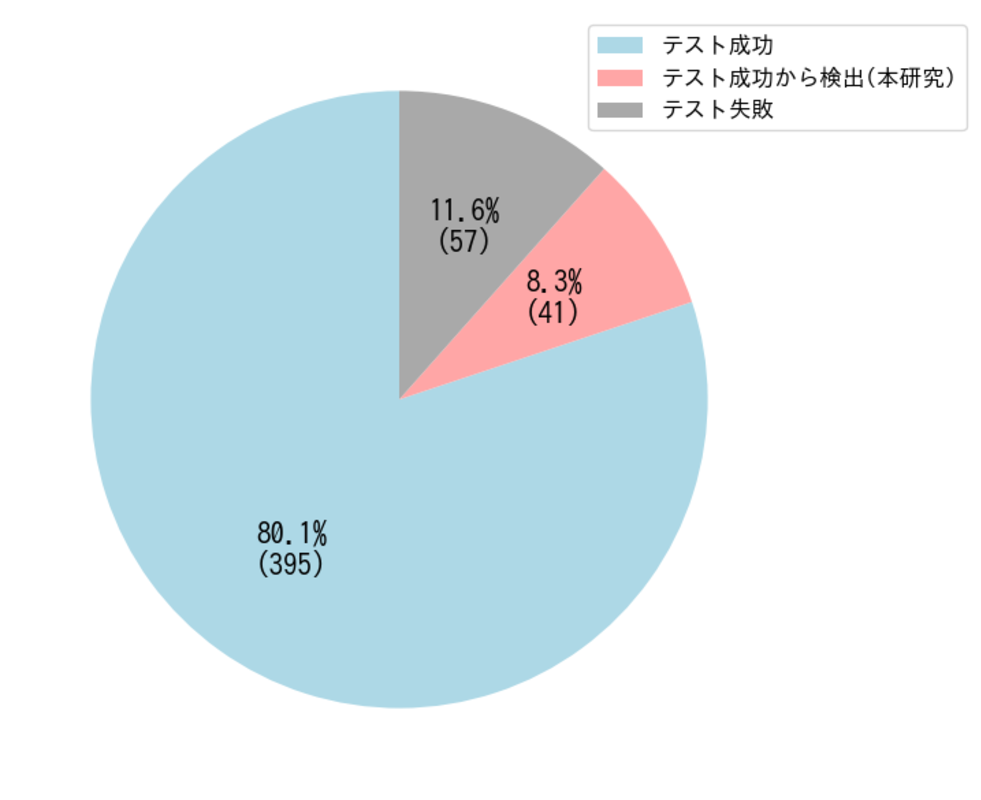
\includegraphics[width=1.0\linewidth]{@BSthesis2024_Iida/BSthesis2024_Iida_fig/RQ2_pie_chart.pdf}}
% \caption{uuid@3.4.0...7.0.0-beta.0の円グラフ}
% \label{fig:method-overview}
% \end{figure*}
% %----------------------
%%%%%%%%%%%%%%%%%%%%%%%%%%%%%

% %----------------------
\begin{table}[t]
    \caption{記述パターンにより検出できたクライアント数}
    \label{table:RQ2}
    \centering
     \scalebox{0.9}{
        \begin{tabular}{l|r|r|r}
        \hline
        \begin{tabular}[c]{@{}c@{}}ライブラリ名@\\ 旧バージョン{...}新バージョン\end{tabular} & \begin{tabular}[c]{@{}c@{}}更新後のテスト失敗\\クライアント数\end{tabular} & \begin{tabular}[c]{@{}c@{}}更新後のテスト成功\\クライアント数\end{tabular} & \begin{tabular}[c]{@{}c@{}}記述パターンを含む\\ テスト成功数(割合)\end{tabular}\\ \hline \hline
            uuid@7.0.3...8.0.0-beta.0 & 119 & 314 & 38 (12\%)\\
            uuid@3.4.0...7.0.0-beta.0 & 55 & 435 & 117 (27\%)\\
            globby@8.0.0...8.0.1 & 42 & 86 & 61 (71\%)\\
            meow@3.6.0...4.0.0 & 26 & 128 & 77(60\%) \\
            globby@6.1.0...7.0.0 & 24 & 113 & 81 (72\%)\\
            pump@1.0.3...2.0.0 & 19 & 83 & 46(55\%) \\
            globby@7.1.1...8.0.0 & 16 & 127 & 94(74\%) \\
            vinyl@1.2.0...2.0.0 & 11 & 58 & 42(72\%) \\ \hline
        \end{tabular}
    }
\end{table}

\begin{table}[t]
    \caption{uuid@7.0.3...8.0.0の記述パターンで検出できるクライアントコード例}
    \label{table:uuid8.0.0_matching_sample}
    \centering
    \scalebox{0.70}{
        \begin{tabular}{c|l|l|l}
            \hline
             \multirow{2}{*}{ID} & \multirow{1}{*}{記述パターン(上はライブラリ呼び出し文,} &  \multicolumn{2}{c}{記述パターンで検出できるクライアントのコード例} \\ \cline{3-4}
            &下は時間数呼び出し文)& コード例1 & コード例2 \\ \hline \hline
    
            \multirow{4}{*}{1}&\multirow{1}{*}{\texttt{(?\textless{}variable1\textgreater{}{[}\textbackslash{}w-{]}+) = }} & \texttt{const uuidV1 = require('uuid/v1')} & \multirow{2}{*}{\texttt{const uuid = require('uuid/v4')}}\\ 
            &\texttt{require(["'\`{}]uuid/v4["'\`{}])[\^{}.]*}& \texttt{const uuidV4 = require('uuid/v4')} & \\ \cline{2-4}
            &\multirow{2}{*}{\texttt{variable1()[\^{}.]*}} & \texttt{uuidV1()} & \multirow{2}{*}{\texttt{uuid()}}\\ 
            & & \texttt{uuidV4()} & \\ \hline

            \multirow{2}{*}{2} & \texttt{(?\textless{}variable1\textgreater{}{[}\textbackslash{}w-{]}+) = } & \texttt{const uuidV1 = require('uuid/v1')} & \multirow{2}{*}{\texttt{var uuid = require("uuid/v1")}}\\ 
            &\texttt{require(["'\`{}]uuid/v1["'\`{}])[\^{}.]*}& \texttt{const uuidV4 = require('uuid/v4')} & \\ \cline{2-4}
            &\multirow{2}{*}{\texttt{variable1()[\^{}.]*}} & \texttt{uuidV1()} & \multirow{2}{*}{\texttt{uuid()}}\\ 
            & & \texttt{uuidV4()} & \\ \hline
            
            \multirow{3}{*}{3} & \texttt{import (?\textless{}variable1\textgreater{}{[}\textbackslash{}w-{]}+) } & \multirow{2}{*}{\texttt{import uuidv4 from 'uuid/v4'}} & \multirow{2}{*}{\texttt{import uuidV4 from "uuid/v4"}}\\ 
            & \texttt{from ["'\`{}]uuid/v4["'\`{}][\^{}.]*} & & \\ \cline{2-4}
            &\texttt{variable1()[\^{}.]*} & \texttt{uuidv4()} & \texttt{uuidV4()()}\\ \hline 
        \end{tabular}
    }
\end{table}


\begin{table}[t]
    \caption{検出したテストが成功していたクライアントのテスト内容}
    \label{table:RQ2_test}
    \centering
    \scalebox{0.95}{
        \begin{tabular}{l|r|r|r} 
        \hline
        \multirow{2}{*}{\begin{tabular}{c}ライブラリ名@\\旧バージョン{...}新バージョン\end{tabular}}
        & \multicolumn{3}{c}{記述パターンを含むテスト成功のクライアント数} \\ \cline{2-4}
        & テストを未設定 & 静的テストを設定 & その他テストあり \\ \hline \hline
        uuid@7.0.3...8.0.0-beta.0 & 7 & 2 & 29 \\
        uuid@3.4.0...7.0.0-beta.0 & 9 & 4 & 104 \\
        globby@8.0.0...8.0.1 & 3 & 3 & 55 \\
        meow@3.6.0...4.0.0 & 1 & 0 & 76 \\
        globby@6.1.0...7.0.0 & 2 & 2 & 77 \\
        pump@1.0.3...2.0.0 & 0 & 12 & 34 \\
        globby@7.1.1...8.0.0 & 4 & 3 & 87  \\
        vinyl@1.2.0...2.0.0 & 2 & 0 & 40\\ \hline
        \end{tabular}
    }
\end{table}
%%%%%%%%%%%%%%%%%%%%%%%%%%%%%
\subsection{実験結果}
\noindent\textbf{1.記述パターンを用いたテストが成功したクライアントの検出結果}

各ライブラリのバージョンにおいて,更新後にテストが成功していたクライアントに対して生成した記述パターンが含まれているクライアントを検出した結果を表\ref{table:RQ2}に示す.表\ref{table:RQ2}は,左からライブラリ名とバージョン,更新後にテストが失敗したクライアント数,更新後にテストが成功したクライアント数,更新後のテスト成功の中から記述パターンにより検出されたクライアント数と検出したクライアント数のテスト成功に占める割合を表している.各ライブラリで更新後にテストが成功しているクライアントのうち,本研究で生成した記述パターンにより検出した(テストに失敗しているクライアントと同じ呼び出し文を使用している)クライアントは,それぞれ12\%から74\%も存在していることがわかった.これらのクライアントは,更新後にテストを実行してもテストが成功するため,後方互換性の損失の影響を受けないと判断されるが,実際には影響を受けている可能性が高い.globby@7.1.1...8.0.0のライブラリでは,74\%ものテストが成功しているクライアントで記述パターンが検出でき,後方互換性の損失により影響を受けても気づくことができないクライアントの割合が8組の中で最も多かった.記述パターンで検出することができるクライアントのコード例を表\ref{table:uuid8.0.0_matching_sample}に示す.表\ref{table:uuid8.0.0_matching_sample}の2列目の記述パターンは,3列目と4列目にあるクライアントのコード例を検出できる.また,ID1とID2に対応するクライアントコード例1のように,1つのクライアントのコードが複数の記述パターンで検出される場合もある.

表\ref{table:RQ1}の5列目(検出時に使用された記述パターン種類数)より本研究で生成した記述パターンのうち,一部の記述パターンしかクライアントを検出できなかった.これは,特定のライブラリと関数呼び出し文がテストが成功したクライアントで使用される傾向にあったのではないかと予想される.テストが成功したクライアントの検出に使用されなかった記述パターンに関して,表\ref{table:uuid8.0.0_description pattern}のID8,ID9のような複数の関数が含まれる複雑な記述パターンも存在するため,完全一致しなかった可能性がある.各ライブラリのバージョンにおける実際の後方互換性の損失による影響範囲は,従来研究の更新後にテストが失敗したクライアントに本研究で検出したクライアント数を加算することで得られると考えられる.また,各記述パターンがクライアントに影響を与えるのかを分析するため,更新後のテストの成否の両方を含むクライアントに対して記述パターンを用いて検出を行った.表\ref{table:uuid8.0.0_description pattern}の4列目がuuidライブラリのバージョン8.0.0-beta.0における検出結果である.ID1〜3において,ID1の記述パターンがクライアント全体の20\%(83/433),ID2とID3の記述パターンがクライアント全体の5\%で使用されていた記述パターンであることが確認できた.
\textbf{\newline\newline}
\noindent\textbf{2.検出したクライアントが設定しているテストの調査結果}

テストに失敗しているクライアントと同じ呼び出し文を記述しているにもかかわらず,テストに成功しているクライアントの一部を目視調査し,原因を調べた.その結果,検出したクライアントには,以下のようなテストが不十分なクライアントを確認した.

\begin{itemize}
\item クライアントにテストが存在しない
\item standardやeslintのような静的テストのみを設定している
\item テストがライブラリ使用箇所を通過していない
\item テストがライブラリの使用箇所を通過しているが,実行結果の中身まで確認していない
\end{itemize}

さらに,テストを設定していないクライアントとstandardやeslintのような静的テストのみを設定しているクライアントを調査した.表\ref{table:RQ2_test}は,記述パターンによって検出できたテストが成功していたクライアントがpackage.jsonに指定していたテストの調査を行なった結果であり,テストを未設定,eslintやstandardのような静的テストのみを設定,その他のテストを設定しているクライアント数を表す.結果よりテストを設定していないまたは静的テストのみを設定しているクライアントを記述パターンによって影響を受ける可能性があると検出できた.また,その他のテストを設定しているクライアントには,テストがライブラリを通過していないまたはライブラリからの戻り値を詳細に検証していないクライアントが含まれると予想できる.テスト不十分なクライアントは,テストが成功しているため後方互換性の損失の影響を把握できないが,本手法が提案する記述パターンを用いることでクライアントのテスト結果のみで判断するよりも後方互換性の損失の影響を受ける可能性の高いクライアントを正確に把握できると考えられる.
\subsection{結果のまとめ}
記述パターンを含むテストが成功したクライアントを検出した結果,各ライブラリのバージョンのテストが成功したクライアントのうち,それぞれ12\%から74\%が検出された.これらのクライアントは,テストが失敗したクライアントと同じライブラリの実装方法をしているため,後方互換性の損失の影響を受けている可能性が高いが,テストが不十分であったため影響に気づけないものであると考えられる.本研究における後方互換性の損失の影響は従来研究の更新後にテストが失敗したクライアントに本研究で検出したクライアントを足したものであると考えられる.また,検出したクライアントの一部を目視調査した結果,テスト不十分なクライアントの要因が確認できたことから提案手法はテストが不十分な場合でも後方互換性の損失の影響範囲を把握することに役立つと期待できる.


%%%%%%%%%%%%%%%%%%%%%%%%%%%%%
\chapter{考察}\label{sec:discussion}
\section{記述パターンの有用性と生成できなかったクライアントの理由}

RQ1の結果では,テストが失敗したクライアントから記述パターンをクライアントのコードから自動生成することができた.記述パターンは,ライブラリ開発者が施した変更によって更新後にエラーが発生するようになった実装方法である.記述パターンには,ライブラリがリリース時に更新後にエラーになる実装方法として周知している実装方法と周知していない実装方法の両方を含んでいることを確認した.周知されていない実装方法を生成できた理由としてクライアントがライブラリの意図しない多様な利用方法をしているためであると予想される.特に周知されていない実装方法に関してライブラリ開発者が意図した変更であれば更新時に公開する文書に記載して注意を促すべきであり,意図しない影響であれば原因の特定やバグの修正をするというような対処が必要になるため,有用であると考える.周知している部分に関しても認識が合っていることの確認や文書に実装方法の具体例を載せたい場合に役立つため,ライブラリ開発者のコスト削減につながると考えている.

本研究では,記述パターンを生成できなかったクライアントも存在している.具体的にクライアントのコードで抽象構文木を作成できない,mockを使用しているためクライアントからライブラリと関数の呼び出し文を全て抽出できないという場合があり,更新後にエラーになる実装方法を取り逃がす危険があるため本研究では除外している.除外している実装方法のクライアントの記述パターンを取れていないため,記述パターン数の低下や検出における取りこぼしに影響すると予想される.表\ref{table:RQ2_test}は,テストが失敗したクライアントから生成できた記述パターンをもとにテストが失敗したクライアントを検出した結果である.検出した結果,記述パターン生成に使用したクライアントは全て検出できたことに加え,一部のファイルを抽象構文木に変換できないため除外していたクライアントが検出された.これにより,テストが失敗したクライアントのうち,65\%から100\% を網羅していることを確認した.

\section{記述パターンによるクライアントの検出による貢献}
RQ2では,記述パターンにより各ライブラリのバージョンでそれぞれ12\%から74\%のクライアントを検出でき,記述パターンが後方互換性の損失の影響を受ける可能性のあるクライアントの検出に役立つことが確認できた.これは,\ref{sec:method}章の記述パターンを生成する際に行なっているクライアントの実装方法のうち,振る舞いに影響のない部分の抽象化を含む汎化処理により上手く検出できたと考える.また,検出したクライアントには,テストが不十分なクライアントが含まれることを確認でき,テストが存在しないクライアントでも後方互換性の損失の影響を把握することができる.ライブラリ開発者がbeta版において検出数を確認することで,事前にクライアントへの影響の把握に役立つと考える.

本研究では,検出数が多い要因として関数呼び出し文に引数がある場合に引数の数のみを残して抽象化している.引数の中身の抽象化により引数の内容を考慮できていないため,引数の数が同じでも影響を受けないククライアントを検出している可能性がある.例としてglobbyライブラリでは,第2引数にオプションを設定するが,この内容によって後方互換性の損失の影響を受ける場合と受けない場合が存在する.このような特定の引数の中身が重要になる場合に誤検出が発生する可能性がある.ただし,本研究の手法では,ライブラリと関数の呼び出し文を考慮することで関数に渡す引数まで追跡していなくともimport文やrequire文の実装方法の変更による後方互換性の損失や関数名と引数の数を組から関数の仕様変更または削除に伴う後方互換の損失などの影響を受けるクライアントを検出できている.また,引数を抽象化することで誤検出は発生する可能性はあるが,後方互換性の損失の影響を受けているまたは受けた関数を使用しているクライアントを特定できる点で記述パターンは役立つと考える.

\section{関数呼び出し文の引数の追跡は静的解析で可能か}

本研究では,関数呼び出し文で定義される引数の内容が静的解析で変数の場合に追跡することが困難であるため,引数の数だけを残して抽象化するという方法をとった.ただ,後方互換性の損失には,引数の型やオプションの指定方法の変更が後方互換性を損失する原因となる事例も存在する.本手法では,引数の中身を考慮できていないため,影響を受けない引数を設定しているクライアントでも引数の数が同じならば,影響を受けると検出してしまう可能性がある.引数の追跡は,引数がファイル内外で設定されることやクライアント関数を経由して引数が渡される場合に静的解析で追跡するのが難しいため,考慮していない.引数の変数名,ファイルのパス,ライブラリが使用されたクライアント関数名を考慮することで引数の追跡を静的解析により実現できるのではないかと推測している.具体的には,引数の変数名は,変数名の定義箇所や関係するクライアント関数の特定のために必要であると考えており,ファイルのパスはクライアント関数の呼び出し関係を把握するために使用する.引数の追跡が実現できれば,引数の内容が原因の後方互換性の損失の影響を分析できると考えている.

\section{妥当性の脅威}
\subsection{内的妥当性}
本研究では,従来研究でバージョン更新前にテストが成功し,更新後にテストが失敗したクライアントから記述パターンを生成し,更新後にテストが成功したクライアントで記述パターンを含むものを検出した.ライブラリ関数に設定された引数の数のみを残し,引数の中身を抽象化している.しかし,後方互換性の損失の原因として関数における引数の型や内容が原因の場合が存在するため,検出の部分で後方互換性の損失の影響を受けない引数を設定しているが,引数の数が同じクライアントを誤検出してしまう可能性があると考える.また,呼び出し文の抽出の際にmockのようなimportやrequireによりクライアントが名付けた名前以外で使用される方法についてファイルをまたがることから,利用される場所の特定が困難なため,本研究ではクライアントごと分析対象外としている.これらの要因が考慮できるようになれば,記述パターンとしてを表現できる要素が増えるため,記述パターンの正確性と多様性が高まり検出精度の向上につながると考える.


\subsection{外的妥当性}
本研究では,JavaScriptライブラリのバージョン更新前にテストが成功したクライアントから更新後にテストが失敗したクライアントとテストが成功したクライアントを分析対象とし,記述パターンの作成とそれによるテスト不十分の要因を持つクライアントを検出した.記述パターンの生成には,ライブラリ更新前にテストが成功し,更新後に失敗したクライアントが必要である.そのため,記述パターンの網羅性が検出精度に影響するため,テストが失敗したクライアント数が少ないライブラリのバージョンにおいて予測精度が変化する可能性がある.後方互換性の損失に影響を受けたクライアントを確保できれば,他のライブラリであっても静的解析による記述パターンの生成とクライアントの検出により記述パターンと影響を受けるクライアントを同様に得られると考える.

%%%%%%%%%%%%%%%%%%%%%%%%%%%%%
\chapter{おわりに}\label{sec:conclusion}

本研究では,ライブラリのバージョン更新に伴いテストが失敗した(後方互換性の損失に影響を受けた)クライアントから後方互換性の損失の影響を受けるため更新後にエラーとなる実装方法である記述パターンを生成した.生成した記述パターンが更新後にエラーとなる実装方法であることを利用し,テストが成功したクライアントからテスト不十分により後方互換性の損失の影響を受けている可能性の高いクライアントを検出した.

RQ1では,記述パターンが本研究で分析対象とした8組のライブラリとバージョンの組でそれぞれ2種類から11種類生成することができた.生成した記述パターンには,ライブラリから公開される文書に後方互換性を損失する実装方法として記載されていた実装方法が含まれていた.さらに,記述パターンとしてライブラリの文書に記載されていない実装方法も含まれており,ライブラリ開発者が想定していない可能性のある後方互換性を損失する実装方法を提供できることが示唆された.

RQ2では,生成した記述パターンを用いてテストが成功したクライアントを検出した結果,各ライブラリのバージョンにおけるテストが成功したクライアントのうち,それぞれ12\%から74\%のクライアントが検出された.検出されたクライアントには,テストを未設定,standardやeslintのような静的テストのみを設定,テストが存在するがライブラリ使用箇所通過していないまたは通過しているが戻り値を検証していないというようなテスト不十分な要因が確認できた.また,クライアントの検出においてテスト不十分により後方互換性の損失に気づいていないクライアントを検出可能であるため,クライアントのテスト結果のみを用いる場合と比較して,より正確に後方互換性の損失の影響を把握できると考えられる.

本研究で提案した記述パターンは,ライブラリ開発者がバージョン更新に伴いクライアントがどのような実装方法で後方互換性の損失の影響を受けるのかを把握することが可能となる.また,ライブラリ開発者が後方互換性の損失する実装方法の例を文書に記載することで,クライアントがテストから後方互換性の損失に気づけない場合でも注意を促せるようになることを期待する.

%%%%%%%%%%%%%%%%%%%%%%%%%%%%%%%%%%%%%%%%%%%%%%%%%%%%%%%%%%%%%%%%%%%%%%%%

%%
%% 謝辞
%%
\begin{acknowledgements}
本研究を進めるに当たって,多くの方々から御指導,御協力を賜りました.ここにお世話になった方々へ感謝の意を記させていただきます.
はじめに,指導教員である和歌山大学システム工学部伊原彰紀准教授に対して,厚く御礼申し上げます.研究室配属以降,研究に関する議論や学会発表に向けた論文執筆,ミーティングなどを通じて多くのご指導を賜りました.そして,学会発表や他大学との交流など様々な方々と交流する機会をいただき,研究に対する建設的な助言をいただくとともに見識を深める貴重な経験を積むことができました.先生のご尽力に敬意を表し,心より感謝いたします.

次に,本研究を進めるにあたり,多大なご協力をいただきました和歌山大学システム工学研究部を卒業された前川 大樹氏には,研究相談や論文執筆,発表資料制作で多くのご助言をいただきました.心より感謝申し上げます.

和歌山大学ソーシャルソフトウェア工学研究室の方々には,常日頃から研究に関する数多くのご助言やご協力を数多くいただきました.また,和歌山大学ソーシャルソフトウェア工学研究室
の同期のおかげで研究活動に加え,大学生活においても充実した日々を過ごすことができました.心より感謝いたします.

最後になりましたが,日頃から温かく見守り,支えてくださった家族に,心より感謝いたします.




\end{acknowledgements}

%%%%%%%%%%%%%%%%%%%%%%%%%%%%%%%%%%%%%%%%%%%%%%%%%%%%%%%%%%%%%%%%%%%%%%%%

%%
%% 参考文献

\bibliographystyle{junsrt}
\bibliography{@BSthesis2024_Iida/BSthesis2024_Iida}


%%%%%%%%%%%%%%%%%%%%%%%%%%%%%%%%%%%%%%%%%%%%%%%%%%%%%%%%%%%%%%%%%%%%%%%%

%%
% 付録
%
\appendix

\chapter{記述パターン一覧}

本研究で生成できた記述パターンの一覧をライブラリごとに記載する.表は,ID,本研究で生成した記述パターン,ライブラリによる文書の有無,全クライアントでの検出数(更新後のテストが失敗したクライアントの検出数+更新後にテストが成功したクライアントの検出数)の並びになっている.

%\multirow{2}{*}{なし}  \multirow{2}{*}{あり} %/は\textbackslash  < \textless{} > \textgreater{}
\begin{table}[t]
    \caption{uuid@7.0.3...8.0.0-beta.0の記述パターン}
    \centering
    \scalebox{0.70}{
        \begin{tabular}{c|l|c|r}
        \hline
            ID & \begin{tabular}{c}記述パターン(上はライブラリ呼び出し文,下は時間数呼び出し文)\end{tabular}&  \begin{tabular}{c}文書\\あり/なし\end{tabular} & \begin{tabular}{c}全クライアント\\での検出数\end{tabular} \\ \hline
            \hline 
        
            \multirow{2}{*}{1} & \texttt{(?\textless{}variable1\textgreater{}{[}\textbackslash{}w-{]}+) = require(["'\`{}]uuid/v4["'\`{}])[\^{}.]*} & \multirow{2}{*}{あり} & \multirow{2}{*}{84/433}\\ \cline{2-2}
            & \texttt{variable1()[\^{}.]*} & & \\ \hline

            \multirow{2}{*}{2} & \texttt{(?\textless{}variable1\textgreater{}{[}\textbackslash{}w-{]}+) = require(["'\`{}]uuid/v1["'\`{}])[\^{}.]*} & \multirow{2}{*}{あり} & \multirow{2}{*}{26/433} \\ \cline{2-2}
            & \texttt{variable1()[\^{}.]*} & & \\ \hline

            \multirow{2}{*}{3} & \texttt{import (?\textless{}variable1\textgreater{}{[}\textbackslash{}w-{]}+) from ["'\`{}]uuid/v4["'\`{}][\^{}.]*} & \multirow{2}{*}{あり} & \multirow{2}{*}{21/433} \\ \cline{2-2}
            & \texttt{variable1()[\^{}.]*} & & \\ \hline

            \multirow{2}{*}{4} & \texttt{import (?\textless{}variable1\textgreater{}{[}\textbackslash{}w-{]}+) from ["'\`{}]uuid/v1["'\`{}][\^{}.]*} & \multirow{2}{*}{あり} & \multirow{2}{*}{5/433}  \\ \cline{2-2}
            & \texttt{variable1()[\^{}.]*} & & \\ \hline 
            
            \multirow{2}{*}{5} & \texttt{import * as (?\textless{}variable1\textgreater{}{[}\textbackslash{}w-{]}+) from ["'\`{}]uuid/v4["'\`{}][\^{}.]*} & \multirow{2}{*}{なし}  &  \multirow{2}{*}{5/433} \\ \cline{2-2}
            & \texttt{variable1()[\^{}.]*} & & \\ \hline
            
            \multirow{2}{*}{6} & \texttt{import * as (?\textless{}variable1\textgreater{}{[}\textbackslash{}w-{]}+) from ["'\`{}]uuid/v1["'\`{}][\^{}.]*} & \multirow{2}{*}{なし}  &  \multirow{2}{*}{4/433} \\ \cline{2-2}
            & \texttt{variable1()[\^{}.]*} & & \\ \hline
            
            \multirow{2}{*}{7} & \texttt{(?\textless{}variable1\textgreater{}{[}\textbackslash{}w-{]}+) = require(["'\`{}]uuid/v4["'\`{}] )[\^{}.]*} & \multirow{2}{*}{あり} & \multirow{2}{*}{1/433}  \\ \cline{2-2}
            & \texttt{variable1([\textasciicircum,]*,[\textasciicircum,]*,[\textasciicircum,]*)[\^{}.]*} & & \\ \hline
            
            \multirow{4}{*}{8} & \texttt{(?\textless{}variable1\textgreater{}{[}\textbackslash{}w-{]}+) = require(["'\`{}]uuid/v4["'\`{}])[\^{}.]*} & \multirow{4}{*}{なし} & \multirow{4}{*}{1/433}  \\
            & \texttt{import * as (?\textless{}variable1\textgreater{}{[}\textbackslash{}w-{]}+) from ["'\`{}]uuid/v4["'\`{}][\^{}.]*} & & \\ \cline{2-2}
            & \texttt{variable1([\textasciicircum,]*,[\textasciicircum,]*)[\^{}.]*}& & \\ 
            & \texttt{variable2([\textasciicircum,]*,[\textasciicircum,]*)[\^{}.]*}& & \\ \hline
            
            \multirow{7}{*}{9} & \texttt{(?\textless{}variable1\textgreater{}{[}\textbackslash{}w-{]}+) = require(["'\`{}]uuid["'\`{}])[\^{}.]*} & \multirow{7}{*}{あり} & \multirow{7}{*}{1/433} \\ 
            & \texttt{(?\textless{}variable2\textgreater{}{[}\textbackslash{}w-{]}+) = require(["'\`{}]uuid/v1["'\`{}])[\^{}.]*} & & \\
            & \texttt{(?\textless{}variable3\textgreater{}{[}\textbackslash{}w-{]}+) = require(["'\`{}]uuid/v4["'\`{}])[\^{}.]*} & & \\
            & \texttt{(?\textless{}variable4\textgreater{}{[}\textbackslash{}w-{]}+) = require(["'\`{}]uuid/v5["'\`{}])[\^{}.]*} & & \\ \cline{2-2}
            
            & \texttt{variable2.apply([\textasciicircum,]*,[\textasciicircum,]*)[\^{}.]*}& & \\ 
            & \texttt{variable3.apply([\textasciicircum,]*,[\textasciicircum,]*)[\^{}.]*}& & \\
            & \texttt{variable4.apply([\textasciicircum,]*,[\textasciicircum,]*)[\^{}.]*}& & \\ \hline
        \end{tabular}
    }
\end{table}
 
\begin{table}[t]
    \caption{uuid@3.4.0...7.0.0-beta.0の記述パターン}
    \centering
    \scalebox{0.70}{
        \begin{tabular}{c|l|c|r}
        \hline
            ID & \begin{tabular}{c}記述パターン(上はライブラリ呼び出し文,下は時間数呼び出し文)\end{tabular}&  \begin{tabular}{c}文書\\あり/なし\end{tabular} & \begin{tabular}{c}全クライアント\\での検出数\end{tabular} \\ \hline
            \hline
        
            \multirow{2}{*}{1} & \texttt{(?\textless{}variable1\textgreater{}{[}\textbackslash{}w-{]}+) = require(["'\`{}]uuid/v4["'\`{}])[\^{}.]*} & \multirow{2}{*}{なし} & \multirow{2}{*}{85/490}\\ \cline{2-2}
            & \texttt{variable1()[\^{}.]*} & & \\ \hline

            \multirow{2}{*}{2} & \texttt{(?\textless{}variable1\textgreater{}{[}\textbackslash{}w-{]}+) = require(["'\`{}]uuid["'\`{}])[\^{}.]*} & \multirow{2}{*}{なし} & \multirow{2}{*}{34/490} \\ \cline{2-2}
            & \texttt{variable1()[\^{}.]*} & & \\ \hline

            \multirow{2}{*}{3} & \texttt{import (?\textless{}variable1\textgreater{}{[}\textbackslash{}w-{]}+) from ["'\`{}]uuid["'\`{}][\^{}.]*} & \multirow{2}{*}{なし} & \multirow{2}{*}{26/490} \\ \cline{2-2}
            & \texttt{variable1.v4()[\^{}.]*} & & \\ \hline

            \multirow{2}{*}{4} & \texttt{import (?\textless{}variable1\textgreater{}{[}\textbackslash{}w-{]}+) from ["'\`{}]uuid["'\`{}][\^{}.]*} & \multirow{2}{*}{なし} & \multirow{2}{*}{14/490}  \\ \cline{2-2}
            & \texttt{variable1.v1()[\^{}.]*} & & \\ \hline 
            
            \multirow{3}{*}{5} & \texttt{(?\textless{}variable1\textgreater{}{[}\textbackslash{}w-{]}+) = require(["'\`{}]uuid["'\`{}])[\^{}.]*} & \multirow{3}{*}{\texttt{なし}}  &  \multirow{3}{*}{4/490} \\
            & \texttt{(?\textless{}variable2\textgreater{}{[}\textbackslash{}w-{]}+) = \_interopRequireDefault(variable1)[\^{}.]*} & & \\ \cline{2-2}
            & \texttt{variable2.default.v4()[\^{}.]*} & & \\ \hline
            
            \multirow{2}{*}{6} & \texttt{(?\textless{}variable1\textgreater{}{[}\textbackslash{}w-{]}+) = require(["'\`{}]uuid["'\`{}])[\^{}.]*} & \multirow{2}{*}{\texttt{なし}}  &  \multirow{2}{*}{2/490} \\ \cline{2-2}
            & \texttt{variable1.v4([\textasciicircum,]*,[\textasciicircum,]*,[\textasciicircum,]*)[\^{}.]*} & & \\ \hline

            \multirow{2}{*}{7} & \texttt{import (?\textless{}variable1\textgreater{}{[}\textbackslash{}w-{]}+) from ["'\`{}]uuid["'\`{}][\^{}.]*} & \multirow{2}{*}{\texttt{なし}}  &  \multirow{2}{*}{2/490} \\ \cline{2-2}
            & \texttt{variable1.v4([\textasciicircum,]*,[\textasciicircum,]*} & & \\ \hline
            
            \multirow{3}{*}{8} & \texttt{(?\textless{}variable1\textgreater{}{[}\textbackslash{}w-{]}+) = require(["'\`{}]uuid["'\`{}] )[\^{}.]*} & \multirow{3}{*}{なし} & \multirow{3}{*}{1/490} \\ 
            & \texttt{import (?\textless{}variable2\textgreater{}{[}\textbackslash{}w-{]}+) from ["'\`{}]uuid["'\`{}][\^{}.]*} & & \\ \cline{2-2}
            & \texttt{variable1.v4()[\^{}.]*} & & \\ \hline
            
            \multirow{6}{*}{9} & \texttt{(?\textless{}variable1\textgreater{}{[}\textbackslash{}w-{]}+) = require(["'\`{}]uuid/v5["'\`{}])[\^{}.]*} & \multirow{6}{*}{なし} & \multirow{6}{*}{1/490} \\ 
            & \texttt{(?\textless{}variable2\textgreater{}{[}\textbackslash{}w-{]}+) = require(["'\`{}]uuid/lib/sha1["'\`{}])[\^{}.]*} & & \\
            & \texttt{(?\textless{}variable3\textgreater{}{[}\textbackslash{}w-{]}+) = require(["'\`{}]uuid/lib/bytesToUuid["'\`{}])[\^{}.]*} & & \\ \cline{2-2}
            & \texttt{variable1([\textasciicircum,]*,[\textasciicircum,]*)[\^{}.]*}& & \\ 
            & \texttt{variable2([\textasciicircum,]*)[\^{}.]*}& & \\
            & \texttt{variable3([\textasciicircum,]*)[\^{}.]*}& & \\ \hline

            \multirow{2}{*}{10} & \texttt{import * as (?\textless{}variable1\textgreater{}{[}\textbackslash{}w-{]}+) from ["'\`{}]uuid["'\`{}][\^{}.]*} & \multirow{2}{*}{なし}  &  \multirow{2}{*}{1/490} \\ \cline{2-2}
            & \texttt{variable1()[\^{}.]*} & & \\ \hline

            \multirow{4}{*}{11} & \texttt{(?\textless{}variable1\textgreater{}{[}\textbackslash{}w-{]}+) = require(["'\`{}]uuid["'\`{}])[\^{}.]*} & \multirow{4}{*}{\texttt{なし}}  &  \multirow{4}{*}{1/490} \\
            & \texttt{(?\textless{}variable2\textgreater{}{[}\textbackslash{}w-{]}+) = \_interopRequireDefault(variable1)[\^{}.]*} & & \\ 
            & \texttt{import (?\textless{}variable3\textgreater{}{[}\textbackslash{}w-{]}+) from ["'\`{}]uuid["'\`{}][\^{}.]*} & & \\ \cline{2-2}
            & \texttt{variable3()[\^{}.]*} & & \\ \hline
            
        \end{tabular}
    }
\end{table}

\begin{table}[t]
    \caption{globby@8.0.0...8.0.1の記述パターンの記述パターン}
    \centering
    \scalebox{0.70}{
        \begin{tabular}{c|l|c|r}
        \hline
            ID & \begin{tabular}{c}記述パターン(上はライブラリ呼び出し文,下は時間数呼び出し文)\end{tabular}&  \begin{tabular}{c}文書\\あり/なし\end{tabular} & \begin{tabular}{c}全クライアント\\での検出数\end{tabular} \\ \hline
            \hline
        
            \multirow{2}{*}{1} & \texttt{(?\textless{}variable1\textgreater{}{[}\textbackslash{}w-{]}+) = require(["'\`{}]globby["'\`{}])[\^{}.]*} & \multirow{2}{*}{なし} & \multirow{2}{*}{32/128}\\ \cline{2-2}
            & \texttt{variable1([\textasciicircum,]*)[\^{}.]*} & & \\ \hline

            \multirow{2}{*}{2} & \texttt{(?\textless{}variable1\textgreater{}{[}\textbackslash{}w-{]}+) = require(["'\`{}]globby["'\`{}])[\^{}.]*} & \multirow{2}{*}{なし} & \multirow{2}{*}{31/128}\\ \cline{2-2}
            & \texttt{variable1([\textasciicircum,]*,[\textasciicircum,]*)[\^{}.]*} & & \\ \hline

            \multirow{2}{*}{3} & \texttt{(?\textless{}variable1\textgreater{}{[}\textbackslash{}w-{]}+) = require(["'\`{}]globby["'\`{}])[\^{}.]*} & \multirow{2}{*}{なし} & \multirow{2}{*}{21/128}\\ \cline{2-2}
            & \texttt{variable1.sync([\textasciicircum,]*,[\textasciicircum,]*)[\^{}.]*} & & \\ \hline

            \multirow{2}{*}{4} & \texttt{(?\textless{}variable1\textgreater{}{[}\textbackslash{}w-{]}+) = require(["'\`{}]globby["'\`{}])[\^{}.]*} & \multirow{2}{*}{なし} & \multirow{2}{*}{12/128}\\ \cline{2-2}
            & \texttt{variable1.sync([\textasciicircum,]*)[\^{}.]*} & & \\ \hline

            \multirow{2}{*}{5} & \texttt{import * as (?\textless{}variable1\textgreater{}{[}\textbackslash{}w-{]}+) from ["'\`{}]globby["'\`{}][\^{}.]*} & \multirow{2}{*}{なし}  &  \multirow{2}{*}{6/128} \\ \cline{2-2}
            & \texttt{variable1([\textasciicircum,]*,[\textasciicircum,]*)[\^{}.]*} & & \\ \hline

            \multirow{2}{*}{6} & \texttt{import * as (?\textless{}variable1\textgreater{}{[}\textbackslash{}w-{]}+) from ["'\`{}]globby["'\`{}][\^{}.]*} & \multirow{2}{*}{なし}  &  \multirow{2}{*}{2/128} \\ \cline{2-2}
            & \texttt{variable1.sync([\textasciicircum,]*)[\^{}.]*} & & \\ \hline

            \multirow{2}{*}{7} & \texttt{import (?\textless{}variable1\textgreater{}{[}\textbackslash{}w-{]}+) from ["'\`{}]globby["'\`{}][\^{}.]*} & \multirow{2}{*}{なし}  &  \multirow{2}{*}{2/128} \\ \cline{2-2}
            & \texttt{variable1.sync([\textasciicircum,]*,[\textasciicircum,]*)[\^{}.]*} & & \\ \hline

            \multirow{2}{*}{8} & \texttt{(?\textless{}variable1\textgreater{}{[}\textbackslash{}w-{]}+) = require( ["'\`{}]globby["'\`{}] )[\^{}.]*} & \multirow{2}{*}{なし} & \multirow{2}{*}{2/128}\\ \cline{2-2}
            & \texttt{variable1.sync([\textasciicircum,]*)[\^{}.]*} & & \\ \hline
            
            \multirow{2}{*}{9} & \texttt{(?\textless{}variable1\textgreater{}{[}\textbackslash{}w-{]}+) = require(["'\`{}]globby["'\`{}])[\^{}.]*} & \multirow{2}{*}{なし} & \multirow{2}{*}{1/128}\\ \cline{2-2}
            & \texttt{variable1([\textasciicircum,]*,[\textasciicircum,]*,[\textasciicircum,]*)[\^{}.]*} & & \\ \hline

            \multirow{3}{*}{10} & \texttt{(?\textless{}variable1\textgreater{}{[}\textbackslash{}w-{]}+) = require( ["'\`{}]globby["'\`{}] )[\^{}.]*} & \multirow{3}{*}{なし} & \multirow{3}{*}{1/128}\\ \cline{2-2}
            & \texttt{variable1([\textasciicircum,]*)[\^{}.]*} & & \\ \hline
            & \texttt{variable1([\textasciicircum,]*,[\textasciicircum,]*)[\^{}.]*} & & \\ \hline
            
        \end{tabular}
    }
\end{table}

\begin{table}[t]
    \caption{meow@3.6.0...4.0.0の記述パターンの記述パターン}
    \centering
    \scalebox{0.65}{
        \begin{tabular}{c|l|c|r}
        \hline
            ID & \begin{tabular}{c}記述パターン(上はライブラリ呼び出し文,下は時間数呼び出し文)\end{tabular}&  \begin{tabular}{c}文書\\あり/なし\end{tabular} & \begin{tabular}{c}全クライアント\\での検出数\end{tabular} \\ \hline
            \hline
        
            \multirow{2}{*}{1} & \texttt{(?\textless{}variable1\textgreater{}{[}\textbackslash{}w-{]}+) = require(["'\`{}]meow["'\`{}])[\^{}.]*} & \multirow{2}{*}{あり} & \multirow{2}{*}{80/154}\\ \cline{2-2}
            & \texttt{variable1([\textasciicircum,]*)[\^{}.]*} & & \\ \hline
            
            \multirow{2}{*}{2} & \texttt{(?\textless{}variable1\textgreater{}{[}\textbackslash{}w-{]}+) = require(["'\`{}]meow["'\`{}])[\^{}.]*} & \multirow{2}{*}{あり} & \multirow{2}{*}{8/154}\\ \cline{2-2}
            & \texttt{variable1([\textasciicircum,]*,[\textasciicircum,]*)[\^{}.]*} & & \\ \hline
            
            \multirow{2}{*}{3} & \texttt{(?\textless{}variable1\textgreater{}{[}\textbackslash{}w-{]}+) = require(["'\`{}]meow["'\`{}])[\^{}.]*} & \multirow{2}{*}{あり} & \multirow{2}{*}{3/154}\\ \cline{2-2}
            & \texttt{variable1.showHelp()[\^{}.]*} & & \\ \hline
            
            \multirow{2}{*}{4} & \texttt{(?\textless{}variable1\textgreater{}{[}\textbackslash{}w-{]}+) = require(["'\`{}]meow["'\`{}])[\^{}.]*} & \multirow{2}{*}{あり} & \multirow{2}{*}{3/154}\\ \cline{2-2}
            & \texttt{variable1([\textasciicircum,]*,[\textasciicircum,]*,[\textasciicircum,]*)[\^{}.]*} & & \\ \hline
            
            \multirow{2}{*}{5} & \texttt{(?\textless{}variable1\textgreater{}{[}\textbackslash{}w-{]}+) = require(["'\`{}]meow["'\`{}])(require(["'\`{}]./help["'\`{}])[\^{}.]*} & \multirow{2}{*}{あり} & \multirow{2}{*}{2/154}\\ \cline{2-2}
            & \texttt{variable1.showHelp()[\^{}.]*} & & \\ \hline
        \end{tabular}
    }
\end{table}

\begin{table}[t]
    \caption{globby@6.1.0...7.0.0の記述パターンの記述パターン}
    \centering
    \scalebox{0.80}{
        \begin{tabular}{c|l|c|r}
        \hline
            ID & \begin{tabular}{c}記述パターン(上はライブラリ呼び出し文,下は時間数呼び出し文)\end{tabular}&  \begin{tabular}{c}文書\\あり/なし\end{tabular} & \begin{tabular}{c}全クライアント\\での検出数\end{tabular} \\ \hline
            \hline
        
             \multirow{2}{*}{1} & \texttt{(?\textless{}variable1\textgreater{}{[}\textbackslash{}w-{]}+) = require(["'\`{}]globby["'\`{}])[\^{}.]*} & \multirow{2}{*}{なし} & \multirow{2}{*}{33/137}\\ \cline{2-2}
            & \texttt{variable1([\textasciicircum,]*)[\^{}.]*} & & \\ \hline

            \multirow{2}{*}{2} & \texttt{(?\textless{}variable1\textgreater{}{[}\textbackslash{}w-{]}+) = require(["'\`{}]globby["'\`{}])[\^{}.]*} & \multirow{2}{*}{なし} & \multirow{2}{*}{32/137}\\ \cline{2-2}
            & \texttt{variable1([\textasciicircum,]*,[\textasciicircum,]*)[\^{}.]*} & & \\ \hline

            \multirow{2}{*}{3} & \texttt{(?\textless{}variable1\textgreater{}{[}\textbackslash{}w-{]}+) = require(["'\`{}]globby["'\`{}])[\^{}.]*} & \multirow{2}{*}{なし} & \multirow{2}{*}{26/137}\\ \cline{2-2}
            & \texttt{variable1.sync([\textasciicircum,]*,[\textasciicircum,]*)[\^{}.]*} & & \\ \hline

            \multirow{2}{*}{4} & \texttt{(?\textless{}variable1\textgreater{}{[}\textbackslash{}w-{]}+) = require(["'\`{}]globby["'\`{}])[\^{}.]*} & \multirow{2}{*}{なし} & \multirow{2}{*}{16/137}\\ \cline{2-2}
            & \texttt{variable1.sync([\textasciicircum,]*)[\^{}.]*} & & \\ \hline

            \multirow{2}{*}{5} & \texttt{import (?\textless{}variable1\textgreater{}{[}\textbackslash{}w-{]}+) from ["'\`{}]globby["'\`{}][\^{}.]*} & \multirow{2}{*}{なし} & \multirow{2}{*}{3/137}\\ \cline{2-2}
            & \texttt{variable1.sync([\textasciicircum,]*)[\^{}.]*} & & \\ \hline

            \multirow{2}{*}{6} & \texttt{import \* as (?\textless{}variable1\textgreater{}{[}\textbackslash{}w-{]}+) from ["'\`{}]globby["'\`{}][\^{}.]*} & \multirow{2}{*}{なし} & \multirow{2}{*}{2/137}\\ \cline{2-2}
            & \texttt{variable1.sync([\textasciicircum,]*)[\^{}.]*} & & \\ \hline

            \multirow{2}{*}{7} & \texttt{(?\textless{}variable1\textgreater{}{[}\textbackslash{}w-{]}+) = require(["'\`{}]globby["'\`{}])[\^{}.]*} & \multirow{2}{*}{なし} & \multirow{2}{*}{1/137}\\ \cline{2-2}
            & \texttt{variable1.sync([\textasciicircum,]*,[\textasciicircum,]*)[\^{}.]*} & & \\ \hline
        \end{tabular}
    }
\end{table}

\begin{table}[t]
    \caption{pump@1.0.3...2.0.0の記述パターンの記述パターン}
    \centering
    \scalebox{0.70}{
        \begin{tabular}{c|l|c|r}
        \hline
            ID & \begin{tabular}{c}記述パターン(上はライブラリ呼び出し文,下は時間数呼び出し文)\end{tabular}&  \begin{tabular}{c}文書\\あり/なし\end{tabular} & \begin{tabular}{c}全クライアント\\での検出数\end{tabular} \\ \hline
            \hline
        
               \multirow{2}{*}{1} & \texttt{(?\textless{}variable1\textgreater{}{[}\textbackslash{}w-{]}+) = require(["'\`{}]pump["'\`{}])[\^{}.]*} & \multirow{2}{*}{なし} & \multirow{2}{*}{62/102}\\ \cline{2-2}
            & \texttt{variable1([\textasciicircum,]*,[\textasciicircum,]*)[\^{}.]*} & & \\ \hline

            \multirow{2}{*}{2} & \texttt{(?\textless{}variable1\textgreater{}{[}\textbackslash{}w-{]}+) = require(["'\`{}]pump["'\`{}])[\^{}.]*} & \multirow{2}{*}{なし} & \multirow{2}{*}{1/102}\\ \cline{2-2}
            & \texttt{variable1.apply([\textasciicircum,]*,[\textasciicircum,]*)[\^{}.]*} & & \\ \hline
        \end{tabular}
    }
\end{table}

\begin{table}[t]
    \caption{globby@7.1.1...8.0.0の記述パターンの記述パターン}
    \centering
    \scalebox{0.70}{
        \begin{tabular}{c|l|c|r}
        \hline
            ID & \begin{tabular}{c}記述パターン(上はライブラリ呼び出し文,下は時間数呼び出し文)\end{tabular}&  \begin{tabular}{c}文書\\あり/なし\end{tabular} & \begin{tabular}{c}全クライアント\\での検出数\end{tabular} \\ \hline
            \hline
        
            \multirow{2}{*}{1} & \texttt{(?\textless{}variable1\textgreater{}{[}\textbackslash{}w-{]}+) = require(["'\`{}]globby["'\`{}])[\^{}.]*} & \multirow{2}{*}{なし} & \multirow{2}{*}{36/143}\\ \cline{2-2}
            & \texttt{variable1([\textasciicircum,]*,[\textasciicircum,]*)[\^{}.]*} & & \\ \hline

            \multirow{2}{*}{2} & \texttt{(?\textless{}variable1\textgreater{}{[}\textbackslash{}w-{]}+) = require(["'\`{}]globby["'\`{}])[\^{}.]*} & \multirow{2}{*}{なし} & \multirow{2}{*}{36/143}\\ \cline{2-2}
            & \texttt{variable1([\textasciicircum,]*)[\^{}.]*} & & \\ \hline

            \multirow{2}{*}{3} & \texttt{(?\textless{}variable1\textgreater{}{[}\textbackslash{}w-{]}+) = require(["'\`{}]globby["'\`{}])[\^{}.]*} & \multirow{2}{*}{なし} & \multirow{2}{*}{26/143}\\ \cline{2-2}
            & \texttt{variable1.sync([\textasciicircum,]*,[\textasciicircum,]*)[\^{}.]*} & & \\ \hline

            \multirow{2}{*}{4} & \texttt{(?\textless{}variable1\textgreater{}{[}\textbackslash{}w-{]}+) = require(["'\`{}]globby["'\`{}])[\^{}.]*} & \multirow{2}{*}{なし} & \multirow{2}{*}{12/143}\\ \cline{2-2}
            & \texttt{variable1.sync([\textasciicircum,]*)[\^{}.]*} & & \\ \hline

            \multirow{2}{*}{5} & \texttt{import (? \textless{}variable1\textgreater{}{[}\textbackslash{}w-{]}+) from ["'\`{}]globby["'\`{}][\^{}.]*} & \multirow{2}{*}{なし} & \multirow{2}{*}{11/143}\\ \cline{2-2}
            & \texttt{variable1([\textasciicircum,]*,[\textasciicircum,]*)[\^{}.]*} & & \\ \hline

        \end{tabular}
    }
\end{table}

\begin{table}[t]
    \caption{viny@1.2.0...2.0.0の記述パターンの記述パターン}
    \centering
    \scalebox{0.70}{
        \begin{tabular}{c|l|c|r}
        \hline
            ID & \begin{tabular}{c}記述パターン(上はライブラリ呼び出し文,下は時間数呼び出し文)\end{tabular}&  \begin{tabular}{c}文書\\あり/なし\end{tabular} & \begin{tabular}{c}全クライアント\\での検出数\end{tabular} \\ \hline
            \hline
        
            \multirow{2}{*}{1} & \texttt{(?\textless{}variable1\textgreater{}{[}\textbackslash{}w-{]}+) = require(["'\`{}]vinyl["'\`{}])[\^{}.]*} & \multirow{2}{*}{なし} & \multirow{2}{*}{52/69}\\ \cline{2-2}
            & \texttt{new variable1([\textasciicircum,]*)[\^{}.]*} & & \\ \hline

            \multirow{7}{*}{2} & \texttt{import (? \textless{}variable1\textgreater{}{[}\textbackslash{}w-{]}+) from ["'\`{}]vinyl["'\`{}][\^{}.]*} & \multirow{7}{*}{なし} & \multirow{7}{*}{1/69}\\ 
            & \texttt{import (? \textless{}variable2\textgreater{}{[}\textbackslash{}w-{]}+) from ["'\`{}]vinyl/lib/isBuffer["'\`{}][\^{}.]*} & & \\
            & \texttt{import (? \textless{}variable3\textgreater{}{[}\textbackslash{}w-{]}+) from ["'\`{}]vinyl/lib/isStream["'\`{}][\^{}.]*} & & \\
            & \texttt{import (? \textless{}variable4\textgreater{}{[}\textbackslash{}w-{]}+) from ["'\`{}]vinyl/lib/isNull["'\`{}][\^{}.]*} & & \\ \cline{2-2}
            & \texttt{variable2([\textasciicircum,]*)[\^{}.]*} & & \\ \cline{2-2}
            & \texttt{variable3([\textasciicircum,]*)[\^{}.]*} & & \\ \cline{2-2}
            & \texttt{variable4([\textasciicircum,]*)[\^{}.]*} & & \\ \hline

        \end{tabular}
    }
\end{table}


% \begin{table}[h]
%     \centering
%     \renewcommand{\arraystretch}{1.3} % 行の高さを少し広げる
%     \begin{tabular}{|c|p{10cm}|c|c|}
%         \hline
%         \textbf{No.} & \textbf{正規表現} & \textbf{判定} & \textbf{確率} \\
%         \hline
%         \multirow{4}{*}{7} & \texttt{(?\textless{}variable1\textgreater{}{[}\textbackslash{}w-{]}+) = require(["'\`{}]uuid/v4["'\`{}] )[\^{}.]*} & \multirow{4}{*}{あり} & \multirow{4}{*}{100} \\
%         & A & & \\  
%         & B & & \\  
%         & C & & \\  
%         \hline
%     \end{tabular}
%     \caption{正規表現のテスト表}
% \end{table}



% \begin{table}[t]
%     \caption{表のもと}
%     \label{table_sample}
%     \centering
%     \scalebox{0.70}{
%         \begin{tabular}{c|l|r|r|r} 
%             \hline
%             \multirow{2}{*}{a} & b  & \multirow{2}{*}{c} & \multirow{2}{*}{d} & \multirow{2}{*}{e}\\ \cline{2-2}
%             & b & & & \\ \hline
%         \end{tabular}   
%     }
% \end{table}

%%%%%%%%%%%%%%%%%%%%%%%%%%%%%%%%%%%%%%%%%%%%%%%%%%%%%%%%%%%%%%%%%%%%%%%%

\end{document}